\documentclass[11pt, a4paper, twoside, frenchb]{book}
\usepackage{styles}

\title{Développement d'une application web collaborative utilisant la programmation réactive-fonctionnelle}
\author{Bastien Clément}
\date{\today}

\usepackage{tikz}
\usetikzlibrary{graphs, graphdrawing}
\usegdlibrary{layered}

%\includeonly{tex/art}

\begin{document}

\maketitle
\tableofcontents

\chapter{Introduction}

\section{Programmation réactive-fonctionnelle}
\section{Objectifs}

\section{Technologies utilisées}

\begin{enumerate}
	\item \textbf{Web Components}: un ensemble d'APIs de la plateforme web destiné à permettre de construire simplement des composants réutilisables et portables grâce au support natif de la technologie dans les navigateurs web modernes. \textit{Web Components} est le regroupement de quatre spécifications plus ciblées:
	\begin{itemize}
		\item \textbf{Custom Elements}: cette première spécification défini une API pour la définition de nouveau élément DOM. En pratique, cela se traduit par la capacité à créer de nouvelle balise HTML reconnue par le navigateur et d'y associer des comportements spécifiques. Il est également possible d'étendre une balise existante selon une forme d'héritage, mais cette fonctionnalité n'est pas exploitée dans ce travail
		
		\item \textbf{Shadow DOM}: défini un mécanisme permettant d'encapsuler un sous-arbre DOM et des styles CSS associés afin de les rendre invisibles de l'extérieur de l'élément hôte. Ce système est largement utilisé pour réaliser l'implémentation interne des éléments personnalisés et limiter ainsi les risques de conflits avec les autres éléments présents dans le document. De plus, les styles CSS placés dans un sous-arbre caché ne peuvent affecter que les éléments de ce sous-arbre, limitant ainsi leur portée.
		
		\item \textbf{HTML Imports}: défini un mécanisme permettant d'importer un document HTML dans un autre document. Dans le cadre de ce travail, cette technologie ne sera pas utilisée. Les composants sont en effet définis entièrement en \textit{Scala.js} et sont donc distribués avec le fichier script compilé de l'application et non dans des documents HTML séparés.
		
		\item \textbf{HTML Template}: défini l'élément HTML \code{<template>} permettant la définition de fragment de document inactifs\footnote{Les images contenues dans ce fragment de document ne sont pas chargées, les scripts ne sont pas exécutés, etc.} qui pourront être instanciés dynamiquement par un script à l'exécution.
	\end{itemize}

	\item \textbf{Scala.js}: ...
\end{enumerate}

\part[Bibliothèque réactive-fonctionnelle]{Bibliothèque réactive-fonctionnelle \\
	\vspace{1cm} {\normalfont Xuen}}
\chapter{Signaux}

\section{Motivations}

La construction d'interfaces utilisateur met en évidence la problématique de la gestion des interactions et du maintient de la cohérence des informations présentées. En effet, les actions effectuées par l'utilisateur modifient l'état du logiciel et requièrent alors une actualisation de l'affichage. Lorsque l'interface devient complexe, maintenir une cohérence globale présente une difficulté de plus en plus importante. Le problème est exacerbé lorsque les modifications de l'état ne proviennent pas uniquement de l'utilisateur mais peuvent également survenir par l'action de processus asynchrones tel qu'une tâche de fond ou une connexion réseau.

La séparation classique Modèle-Vue-Contrôleur repose généralement la notion d'\emph{Observable} et d'\emph{Observateur} pour lier Vue et Modèle. Ce concept présente cependant de multiples inconvénients tel que la promotion d'effets de bord, une diminution de l'encapsulation, une verbosité excessive; le rendant ainsi fastidieux à l'utilisation et sujet à erreurs \cite{odersky2012}.

Ingo Maier et Martin Odersky proposent ainsi une approche plus fonctionnelle et composable avec la bibliothèque \emph{Scala.React} \cite{scala-react} avec entre autres la notion de signal: une valeur pouvant varier avec le temps. Cependant les signaux ne sont qu'un des multiples outils mis à disposition et l'utilisation de la bibliothèque se révèle être excessivement complexe, même dans les cas les plus simples \cite[\small Related~Work]{scala.rx}.

\textit{La complexité de Scala.React est introduite par une implémentation thread-safe destinée aux application de type fat-client dans un environnement JVM local. À l'inverse Scala.rx est développée avec des systèmes tels que JavaScript où la concurrence n'est pas un problème.}

Partant de ce constat, Li Haoyi a ainsi développé \emph{Scala.Rx} \cite{scala.rx}: une réimplémentation simplifiée du concept de signaux avec une emphase sur la simplicité, à la fois au niveau de la conception que de l'utilisation. Cependant, par simplicité, plusieurs limitations ont été volontairement imposées et se révèlent être particulièrement gênantes dans le cadre de ce projet.

Xuen implémente ainsi un concept de signaux largement basés sur ceux de \emph{Scala.Rx}, mais dont les fonctionnalités ont été spécifiquement adaptées à leurs utilisation dans le cadre du développement d'interfaces utilisateur et de l'utilisation de données chargées de façon asynchrone.

\section{Spécifications}

\subsection{Définition}
Un \texttt{Signal[T]} représente une information de type \texttt{T} dont la disponibilité ou la valeur peut varier avec le temps. À tout moment, il peut se trouver dans l'un des deux états suivants:
\begin{enumerate}
	\item \texttt{Undefined}: le signal ne possède pas de valeur définie,
	\item \texttt{Defined(value)}: le signal possède actuellement la valeur \texttt{value}
\end{enumerate}

Il peut être vu comme une extension de \texttt{Future[T]}. De façon similaire, il représente la présence ou l'absence d'information au fil du temps, mais à la différence de \texttt{Future}, il est autorisé à changer d'état un nombre arbitraire de fois tandis que l'état d'un \texttt{Future} est figé une fois celui-ci résolu.

Le type \texttt{Signal[T]} est covariant avec son paramètre \texttt{T}. L'interface exposée ne permettant que l'accès à la valeur du signal ou sa transformation par le biais de la construction d'un nouveau signal, une instance \texttt{Signal[B]} est substituable à \texttt{Signal[A]} si \texttt{B <: A}\footnote{\texttt{B <: A} désigne une relation de sous-type (\texttt{B extends A})}.

L'état d'un signal peut être dépendant de l'état d'un ou plusieurs autres signaux. Il constitue alors un signal \emph{enfant} associé à un ensemble de signaux \emph{parents}. Cet ensemble peut varier dynamiquement au fil du temps. Un signal enfant ne peut changer d'état que lorsque au moins l'un des ses signaux parents change d'état.

À l'inverse, un signal qui ne dépend d'aucun autre est appelé une \emph{source}. Le changement d'état d'un signal source ne peut s'opérer que par une mutation explicite, extérieur au système de signaux.

\texttt{Signal} vérifie les trois axiomes des monades \cite{haskell-monad-laws}:
\begin{align*}
Signal(x) \text{ flatMap } f &\equiv f(x) \\
a \text{ flatMap } (x \mapsto Signal(x)) &\equiv a \\
(a \text{ flatMap } f)  \text{ flatMap } g &\equiv
a \text{ flatMap } (x \mapsto f(x)  \text{ flatMap } g) 
\end{align*}
Ici, l'opérateur $\equiv$ désigne une équivalence structurelle: les deux expressions sont substituables sans changer le comportement du programme.

\subsection{Accès à l'état courant}
L'interface d'un signal \texttt{Signal[T]} défini deux méthodes pour accéder à sa valeur courante:
\begin{enumerate}
	\item \textbf{\texttt{Signal.option}}: retourne la valeur courante d'un signal sous la forme d'une \texttt{Option[T]}. C'est une façon sûre d'accéder à l'état du signal quel qu'il soit.
	
	\item \textbf{\texttt{Signal.value}}: retourne la valeur courante du signal (donc une valeur de type \texttt{T}) s'il est défini ou lance une exception\footnote{De type \texttt{UndefinedSignalException}} s'il ne l'est pas. De façon générale, cette méthode est plutôt destinée à être utilisée dans le cadre de la définition de signaux expression (section \ref{sec:sig-expr}) puisque dans ce cas, l'exception est traitée par le constructeur et entraîne la construction d'un signal vide.
\end{enumerate}

Dans le cas où il est nécessaire d'être informé des changements d'états du signal, le mécanisme d'observateur (§~\ref{sec:sig-obs}) peut être utilisé.

\subsection{Pureté et modes d'évaluation} \label{sec:sig-pureness}
Un signal est considéré comme une construction fonctionnelle semi-pure: il n'est dépendant d'aucun état global à l'exception d'autres signaux et ne présente pas d'effets de bords. Ces contraintes s'étendent également aux fonctions utilisées dans leur définition ou transformation par le biais de fonctions telle que \texttt{map} ou \texttt{filter}. Le langage Scala ne permettant pas d'imposer la notion de pureté aux fonction, il est de la responsabilité du développeur de s'assurer que cette contrainte soit respectée.

Cette contrainte découle principalement de l'existence de deux modes d'évaluations pour les signaux qui définissent à quel moment l'état d'un signal enfant doit être calculé après le changement d'état d'un de ses signaux parent:
\begin{enumerate}
	\item \emph{Paresseux}: l'état du signal enfant est réévalué à la demande, lorsque son état courant est accédé et après un changement d'état d'au moins un des ses signaux parents,
	\item \emph{Strict}: l'état du signal enfant est réévalué aussitôt que l'état d'un de ses signaux parent est modifié.
\end{enumerate}

Le mode d'évaluation paresseux est le mode utilisé par défaut pour les signaux. Il offre l'avantage de réduire le nombre d'états à calculer dans le cas où un signal n'est pas accédé aussi fréquemment que son état ne change.

Le mode paresseux n'offre aucune garantie concernant le moment auquel une fonction utilisée comme définition d'un signal ou d'une transformation sera appelée, ni même qu'elle sera un jour appelée. Il est donc particulièrement important que ces fonctions respectent également la contrainte de pureté des signaux pour ne pas introduire des comportements non-déterministes dans l'application.

Le mode strict n'est utilisé que dans les situations où l'événement de changement d'état est significatif en plus de la valeur de ce nouvel état. C'est par exemple le cas de l'opération \texttt{fold} (§ \ref{sec:sig-op-fold}) qui est utilisée pour combiner les états successifs d'un signal parent afin de construire l'état du signal enfant. Dans une telle situation, l'utilisation du mode paresseux rendrait le signal enfant non-déterministe puisque son état serait dépendant de la fréquence à laquelle il est accédé \footnote{Si la fréquence d'accès est inférieure à la fréquence de changement d'état du signal parent, certains états seront \emph{manqués} par l'opération de combinaison passé à \texttt{fold}.}.

De façon générale, l'utilisation sélective du mode d'évaluation stricte conduit à la construction de groupes de signaux à l'intérieur du graphe de dépendances qui sont toujours réévalués simultanément. Cette réévaluation groupée est cependant limitée à une petite partie du graphe et n'implique pas les mêmes coûts de calculs qu'une stratégie d'évaluation stricte qui serait utilisée de façon globale. 

\subsection{Hiérarchie simplifiée}
La figure \ref{fig:sig-simple-hierarchy} présente une version simplifiée de la hiérarchie des signaux. Seules les informations pertinentes à l'utilisation des signaux ont été conservée: les méthodes, interfaces, classes intermédiaires relevant des détails d'implémentation ne sont pas incluses. La hiérarchie complète formée par les signaux est présentée en section \ref{sec:sig-hierarchy}.

\begin{figure}[!h]
	\centering
	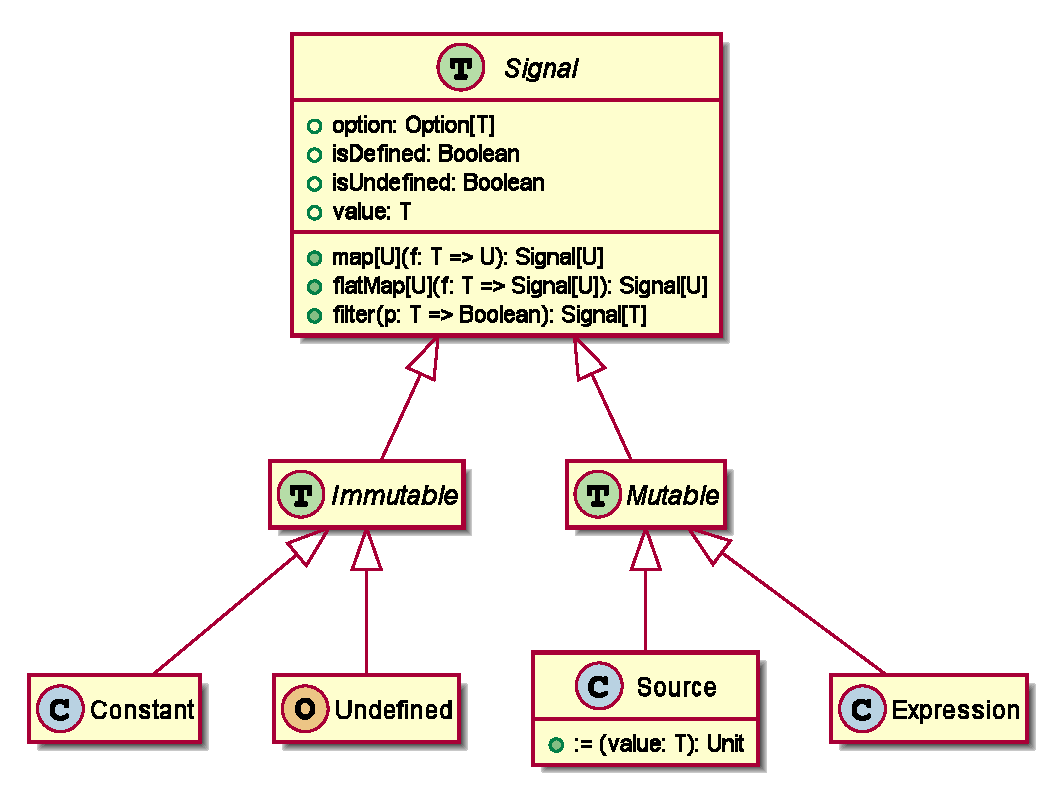
\includegraphics[width=12cm]{img/signals_simple}
	\caption{Hiérarchie simplifiée des signaux}
	\label{fig:sig-simple-hierarchy}	
\end{figure}

Le trait racine \texttt{Signal} est l'interface générique destinée à être manipulée par le développeur, quelque soit le type concret de signal manipulé. Il expose les méthodes nécessaires à l'accès à l'état courant du signal ainsi qu'à la construction de signaux dérivés par transformation. C'est une interface immutable qui ne permet de modifier l'état courant du signal.

La séparation des signaux en deux sous-arbres --- \texttt{Mutable} et \texttt{Immutable} --- capture les différences sémantiques liées à la présence ou l'absence d'une garantie d'immutabilité de l'état d'un signal.

L'intérêt d'un signal dont la valeur ne varie pas peut sembler limité à priori mais se présente lorsqu'une valeur non-signal doit être encapsulée dans un signal afin de satisfaire le système de types. Un tel signal n'a pas de raison de changer d'état au fil du temps, il est alors effectivement immutable. La présence de cette contrainte de façon explicite au niveau de la hiérarchie permet la mise en place d'un certain nombre d'optimisations.

Une instance de la classe \texttt{Constant[T]} est simplement une valeur de type \texttt{T} avec une interface de signal. Un tel signal est toujours dans l'état \emph{défini}.

L'objet singleton \texttt{Undefined} représente quant à lui le signal dont l'état est toujours \emph{indéfini}. Il est généralement référencé à partir de l'objet compagnon du trait \texttt{Signal}: sous la forme \texttt{Signal.undefined}. Puisqu'il n'est jamais défini, il est défini comme une instance de \texttt{Signal[Nothing]}, il est donc par covariance substituable à n'importe quel type de signal \texttt{Signal[T]} \footnote{\texttt{Nothing} est le \emph{bottom type} du système de types en Scala, il est sous-type de tous les types ($\forall \texttt{T}, \texttt{Nothing <: T}$) mais il n'en existe aucune instance.}.

Un signal immutable ne peut être ni \emph{enfant} ni \emph{parent} d'autres signaux. Comme ils ne changent jamais, il n'y a pas de sens de maintenir de graphe de dépendances entre eux. Il n'y aura en effet jamais de propagation de changement d'état à effectuer.

Les opérations de transformation --- \texttt{map}, \texttt{flatMap}, \texttt{filter}, etc. --- appliquées à des signaux constants sont évaluées immédiatement et produisent un nouveau signal constant. Par exemple:

\begin{lstlisting}
val a: Constant[Int] = Constant(2)
val b: Constant[Int] = a.map(_ * 2) // effectuée immédiatement
\end{lstlisting}

\begin{figure}
	\begin{lstlisting}
var i: Int = 0
def f(v: Int): Int = { i += 1; v * 2 }

// Immutable
val a: Constant[Int] = Constant(2)
val b: Constant[Int] = a.map(f)
assert(i == 1) // `f` est évaluée immédiatement

// Mutable
val c: Signal[Int] = Signal(2)
val d: Signal[Int] = c.map(f)
assert(i == 1) // `f` est évaluée de façon paresseuse
assert(d.value == 4) // accès à l'état de `d`, évaluation
assert(i == 2)

// Une sémantique peut en cacher une autre...
val e: Signal[Int] = Constant(2) // typé `Signal`
val f: Signal[Int] = c.map(f)
assert(i == 3)
	\end{lstlisting}
	\caption{Exemple d'évaluation immédiate des transformations}
	\label{fig:constant-eager-transform}
\end{figure}

La figure \ref{fig:constant-eager-transform} illustre ce comportement de façon plus explicite par l'introduction d'effets de bord dans la fonction de transformation utilisée. Cet exemple souligne également l'importance de la pureté des fonctions utilisées en pratique.

Les deux types de signaux mutables, sources (§ \ref{sec:sig-source}) et expressions (§ \ref{sec:sig-expr}), sont décrits plus en détails dans les sections les concernant.

\subsection{Construction}
Un signal est généralement dérivé par transformation de signaux existants. Cependant, dans le cas où un nouveau signal racine doit être construit, deux approches sont disponibles.

La première méthode est l'utilisation des constructeurs offerts par l'objet \texttt{Signal}:

\begin{itemize}
	\item \code{def Signal.apply[T](expr: => T): Signal[T]}
	\item \code{def Signal.define[T](expr: => Option[T]): Signal[T]}
\end{itemize}

L'expression fournie à \texttt{apply} sera évaluée pour déterminer la valeur du signal produit et les dépendances vers d'autres signaux seront automatiquement identifiées. Si l'expression fait référence à l'état d'au moins un signal parent non-constant, un signal de type \texttt{Expression} (§ \ref{sec:sig-expr}) est retourné. Dans le cas où aucun signal parent n'a été accédé, un signal de type \texttt{Constant} est retourné.

La variante \texttt{define} est similaire mais considère une valeur \texttt{None} comme un signal indéfini tandis qu'une valeur \texttt{Some(v)} est considérée comme un signal défini et de valeur \texttt{v}. 

La secondes approche consiste en l'utilisation explicite d'un signal de type \texttt{Source} (§ \ref{sec:sig-source}). 

\subsection{Signal source} \label{sec:sig-source}

Une \texttt{Source[T]} est l'équivalent réactif d'une variable en programmation non-réactive. C'est un conteneur mutable pour une valeur de type \texttt{T}, pouvant être indéfinie. Deux constructeurs sont disponibles selon l'état initial désiré pour la source:

\begin{itemize}
	\item \code{def Source.apply[T](value: T): Source[T]}
	\item \code{def Source.undefined[T]: Source[T]}
\end{itemize}

Une instance de \texttt{Source[T]} offre une méthode de mutation explicite
\begin{center}
	\code{def := (value: T): Unit}
\end{center}
permettant de mettre à jour la valeur contenue dans la source de façon impérative. Cette opération est un changement d'état de la source et provoquera l'invalidation récursive des tous les signaux en dépendant.

Une source est destinée à être utilisées lors de la construction de système hybrides, combinant code impératif basé sur les effets de bords et code fonctionnel. La source est alors un point d'entrée dans le graphe de dépendances des signaux pour la partie de code impérative.

\textit{À ajouter: une opération utilisant une fonction de mutation à partir de l'état courant:}
\begin{lstlisting}
	def ~= (f: T => T): Unit = { this := f(value) }
\end{lstlisting}

\subsection{Signal expression} \label{sec:sig-expr}

Un signal expression est un signal dont la définition est une expression arbitraire. Un tel signal détermine automatiquement ses signaux parents en observant les signaux accédés lors de l'évaluation de l'expression et construit ainsi automatiquement son arbre de dépendances. Si l'un de ces signaux venait à changer, la valeur du signal expression serait recalculée.

Il est construit en passant l'expression de définition au constructeur \texttt{Signal} tel qu'illustré par la figure \ref{fig:signal-expr-init}. La variante \texttt{Signal.define} est similaire à la méthode \texttt{apply}, mais reçoit une expression de type \texttt{Option[T]}. Une évaluation de cette expression produisant la valeur \texttt{None} ou une instance \texttt{Some(v)} conduit respectivement à un état indéfini ou défini du signal.

\begin{figure}[!h]
	\begin{lstlisting}
val a: Signal[Int] = ...
val b: Signal[Int] = ...
val c: Signal[Int] = Signal {
	a.value + b.value
}
	\end{lstlisting}
	\caption{Déclaration d'un signal expression}
	\label{fig:signal-expr-init}
\end{figure}

Les parents d'un signal expression sont dynamiques. À chaque évaluation, la liste des parents est vidée puis reconstruite selon l'évaluation actuelle. De cette façon, les dépendances sont toujours le plus précises possible et les invalidation inutiles sont évitées. Ceci est particulièrement important dans le cas de signaux contenant des branches et donc un ensemble de dépendances dynamiques selon l'état d'autres signaux.

Dans l'exemple de la figure \ref{fig:signal-expr-branches}, le signal construit ne dépend de \texttt{b} que si la valeur du signal \texttt{a} est \texttt{false}. Dans le cas contraire, il est dépendant de \texttt{c}. Dans tous les cas, une dépendance est créée vers le signal \texttt{a}.

\begin{figure}[!h]
	\begin{lstlisting}
Signal {
	if (a.value) b.value else c.value
}
	\end{lstlisting}
	\caption{Définition d'un signal expression avec branches}
	\label{fig:signal-expr-branches}
\end{figure}

Selon la situation, l'usage d'une expression pour définir un signal peut se révéler plus simple que la combinaison de nombreuses opérations de transformations élémentaires pour composer le comportement attendu.

Dans les cas les plus complexes, principalement lors de l'utilisation de structures de contrôles tel que des branches conditionnelles, des opérations de \emph{pattern matching} ou des boucles, une expression permet une définition concise et atomique du signal tandis que pour obtenir un résultat équivalent à l'aide des opérateurs de transformation, une longue chaîne de transformations successives, considérablement plus difficile à comprendre, serait nécessaire.

À l'inverse, dans les cas plus simples, une opération de transformation permet de réutiliser un \emph{pattern} de transformation établi, étant alors à la fois plus concis et mentalement plus simple puisqu'il utilise une sémantique clairement établie et commune.

\subsubsection{Contraintes des expressions}

Les signaux doivent être considérés comme des constructions semi-pure d'un point de vue fonctionnel (§~\ref{sec:sig-pureness}). Il est ainsi important que l'expression utilisée comme définition respecte ce principe en ne provoquant aucun effet de bord et en ne dépendant d'aucune valeur mutable qui ne serait pas un signal. En effet, si une valeur mutable non-signal est référencée par une expression, l'état résultant du signal est alors dépendant de l'instant d'évaluation pour lequel aucune garantie n'est fournie.

Il est aussi important que l'évaluation d'une expression s'effectue de façon synchrone. En effet la liste de dépendances du signal est construite lors de l'évaluation de l'expression. Si un signal parent est accédé de façon asynchrone ou \emph{lazy}, la dépendance ne sera pas identifiée et le signal ne sera pas correctement invalidé en cas de changement d'état de ce signal parent.

Les deux principaux suspects à considérer sont \texttt{Future} et \texttt{Stream}. Le premier pour le délai qu'il introduit dans l'évaluation de sa valeur, le second pour sa sémantique \emph{lazy}.

Il est intéressant de noter que la seule observation du paramètre de type du signal permet d'identifier un potentiel problème. En effet un signal de type \texttt{Signal[Int]} dont la définition impliquerait l'utilisation d'une instance de \texttt{Stream} n'est pas un souci; une fois la valeur finale de type \texttt{Int} produite, l'ensemble des éléments pertinents du flux auront été consommés de façon synchrone. Le principe s'applique de façon similaire à l'opération \texttt{Option.orElse} pour laquelle le paramètre est passé \emph{by name}.

À l'inverse, un signal \texttt{Signal[Stream[Int]]} expose l'instance de \texttt{Stream} utilisée. Dans une telle situation, si le calcul d'un élément du flux requiert l'accès à un autre signal, aucune relation de dépendance ne sera établie. Des types de signaux tels que \texttt{Signal[Stream[A => B]]}, \texttt{Signal[Future[A]]} voir même \texttt{Signal[A => B]} indiquent un risque important ne pas respecter la contrainte de synchronisme.

\subsection{Opérateurs de transformations}
Dans les exemples ci-dessous, les opérations sont supposées appliquées à une instance de type \texttt{Signal[T]}, \texttt{T} faisant ainsi référence au type d'élément contenu dans le signal original. Seules les opérateurs les plus courants et ceux utilisées par le compilateur Scala lors de la compilation d'une compréhension \texttt{for} sont traités ici. La Scaladoc du projet contient une liste exhaustive des opérations disponibles.

\subsubsection{Opérateur de transformation simple (\texttt{map})}

\begin{itemize}
	\item \code{def map[U](f: T=>U): Signal[U]}
\end{itemize}

La fonction \texttt{map} effectue une opération de transformation simple sur la valeur d'un signal en appliquant la fonction \texttt{f} à la valeur courante du signal et retournant un nouveau signal contenant en tout temps le résultat de cette transformation. En d'autre termes, lorsque l'état du signal original change, la fonction \texttt{f} est réévaluée avec la nouvelle valeur du signal parent et le signal enfant est mis à jour.

Si le signal d'origine est indéfini, la fonction \texttt{f} n'est pas appliquée et le signal enfant prend également l'état indéfini.

\begin{figure}[h]
	\begin{lstlisting}
val a: Signal[Int] = Source(4)
val b: Signal[Double] = a.map(Math.sqrt(_)) // b.value -> 2.0
a := 9 // b.value -> 3.0

val c: Signal[_] = Signal.undefined // `c` est indéfini
val d: Signal[_] = c.map(value => ???)
d.option == None // la fonction passée à `map` n'est jamais évaluée
	\end{lstlisting}
	\caption{Exemple d'utilisation de \texttt{map}}
\end{figure}

\subsubsection{Opérateur de sélection (\texttt{flatMap})}

\begin{itemize}
	\item \code{def flatMap[U](f: T=>Signal[U]): Signal[U]}
\end{itemize}

Dans le cas des signaux, \texttt{flatMap} implémente une opération de sélection: étant donné un signal \texttt{a} de type \texttt{Signal[T]} et une transformation sous la forme d'une fonction \texttt{f: T => Signal[U]}, la fonction \texttt{f} est appliquée à la valeur actuelle du signal \texttt{a} afin d'obtenir un second signal \texttt{b} de type \texttt{Signal[U]} et retourne un troisième signal \texttt{c} également de type \texttt{Signal[U]} dont la valeur est en tout temps égale à celle du signal \texttt{b}. La fonction \texttt{f} est réévaluée à chaque changement d'état du signal \texttt{a} afin de définir un nouveau signal de référence \texttt{b}.

Si le signal \texttt{a} est indéfini, la fonction \texttt{f} n'est pas appliquée et le signal \texttt{c} est également considéré indéfini.

La fonction \texttt{flatMap}\footnote{\emph{bind} en Haskell, ou \texttt{>>=}} est la fonction universelle de transformation des monades. Elle est suffisamment générale pour permettre de définir toutes les autres fonctions de transformation comme des cas particuliers de \texttt{flatMap}. Par exemple, la transformation \texttt{a.map(f)} peut également s'écrire  sous la forme \texttt{a.flatMap(value => Constant(f(value))}.

\begin{figure}[h]
	\begin{lstlisting}
val choice: Signal[Int] = ...
def selectSignal(choice: Int): Signal[T] = ...
// L'état de `c` est identique à celui du signal retourné par `selectSignal` pour la valeur courante de `choice`
val c: Signal[T] = choice.flatMap(selectSignal)
	\end{lstlisting}
	\caption{Exemple d'utilisation de \texttt{flatMap}}
\end{figure}

\subsubsection{Opérateur de filtrage (\texttt{filter})}

\begin{itemize}
	\item \code{def filter(p: T=>Boolean): Signal[T]}
\end{itemize}

La fonction \texttt{filter} effectue une opération de filtrage d'un signal en appliquant un prédicat \texttt{p} à la valeur courante du signal et retournant un nouveau signal de même valeur si le prédicat est vérifié, ou un signal indéfini si le prédicat n'est pas vérifié.

\begin{figure}[h]
	\begin{lstlisting}
	val a: Signal[Int] = Source(4)
	val b: Signal[Int] = a.filter(_ % 2 == 0) // b.option -> Some(4)
	a := 5 // b.option -> None, b.value -> UndefinedSignalException
	\end{lstlisting}
	\caption{Exemple d'utilisation de \texttt{filter}}
\end{figure}

\subsubsection{Opérateur de combinaison (\texttt{fold} / \texttt{reduce})} \label{sec:sig-op-fold}

\begin{itemize}
	\item \code{def fold[U](a: U)(f: (U, T)=>U): Signal[U]}
	\item \code{def reduce[U >: T](f: (U, T)=>U): Signal[U]}
\end{itemize}

L'opérateur \texttt{fold} permet l'introduction d'un effet de \emph{mémoire} aux signaux. Il prend en paramètre un \emph{accumulateur initial} \texttt{a} de type \texttt{U} et une fonction de combinaison \texttt{f: (U, T) => U} permettant d'associer la valeur courante du signal à cet état pour produire un \emph{accumulateur courant}, également de type \texttt{U}, qui sera alors la valeur du signal produit par l'opérateur.

Lors d'un changement d'état du signal initial, l'\emph{accumulateur antérieur} est combiné à la nouvelle valeur du signal pour former le nouvel \emph{accumulateur courant}. Si le signal est indéfini la fonction \texttt{f} n'est pas évaluée et l'\emph{accumulateur antérieur} devient l'\emph{accumulateur courant} sans modification. Dans le cas où le signal est initialement indéfini, l'\emph{accumulateur initial} devient l'\emph{accumulateur courant} tel quel.

Le signal retourné par \texttt{fold} est toujours défini.

L'opérateur \texttt{fold} possède la particularité d'être affecté par le mode d'évaluation du signal qu'il produit. En mode paresseux, l'opérateur de combinaison ne serait appliqué que lors de l'accès au signal enfant. Il serait alors possible de \emph{manquer} des changements d'état du signal parent. C'est pourquoi les signaux produits par l'opérateur \texttt{fold} ont toujours un mode d'évaluation strict afin d'obtenir un comportement déterministe et indépendant de la façon dont le signal enfant est utilisé.

À l'inverse de la fonction \texttt{fold} présente sur les collections de la bibliothèque standard Scala qui retourne une unique valeur pour une collection. La fonction \texttt{fold} des signaux retourne également un \texttt{Signal}. Le nom \emph{fold} ne fait ainsi pas référence au passage d'une collection à un élément unique, mais à la combinaison successive des différents \emph{états} du signal parent.

\begin{figure}[h]
	\begin{lstlisting}
val a: Signal[Int] = ...
val s: Signal[Int] = a.fold(0)(_ + _)
// Le signal `s` représente la somme de toutes les valeurs du signal `a`.

val b: Signal[Int] = ...
val m: Signal[Int] = b.fold(0)(_ max _)
// Le signal `m` représente la valeur maximale obtenue par le signal `b`.
	\end{lstlisting}
	\caption{Exemple d'utilisation de \texttt{fold}}
\end{figure}

L'opérateur \texttt{reduce} est une variation de l'opérateur \texttt{fold} dont l'\emph{accumulateur initial} est déterminé implicitement par l'état courant du signal parent. À l'inverse de la transformation \texttt{fold}, si l'état courant du signal parent est indéfini, alors le signal enfant est également indéfini. Dès lors que l'état du signal parent sera défini pour la première fois, l'état du signal enfant ne pourra plus être indéfini.

\begin{figure}[h]
	\begin{lstlisting}
val a: Signal[Int] = ...
val b: Signal[Int] = a.reduce((acc, x) => x)
// La valeur du signal `b` reflète la valeur du signal `a` lorsque celui-ci est défini. Lorsqu'il est indéfini, le signal `b` contient la dernière valeur définie du signal `b`. Si `a` n'a jamais été défini, `b` est indéfini.

val c: Signal[Int] = ...
val d: Signal[Int] = c.reduce(_ max _)
// Similaire à l'exemple correspondant pour `fold`, mais ne suppose pas une valeur intiale de 0. Si `c` représente des nombres négatifs, la version avec `fold` ne serait pas correcte (il faudrait utiliser Int.MinValue).
	\end{lstlisting}
	\caption{Exemple d'utilisation de \texttt{reduce}}
\end{figure}

\textit{À DÉTERMINER: Initialement, une variante \texttt{foldLazy} était envisagée qui produirait un signal avec le mode d'évaluation lazy. Dans quelles situations serait-ce adapté? J'avais initialement en tête des opérateurs tels que \texttt{max} qui ne conserve pas de trace de la séquence observée mais seulement un unique élément. Mais même de tels opérateurs n'ont pas de sens en évaluation paresseuse. L'essence de l'opération \texttt{fold} est de combiner des états successifs, comment cette opération peut-elle avoir un sens si certains états sont manqués de façon non-prévisible?}

\subsubsection{Opérateurs d'encapsulation (\texttt{wrap / unwrap})}

\begin{itemize}
	\item \code{def wrap: Signal[Option[T]]}
	\item \code{def unwrap[U](implicit ev: T <:< Option[U]): Signal[U]}
\end{itemize}

L'opérateur \texttt{wrap} transforme un signal d'origine de type \texttt{T} en un signal de type \texttt{Option[T]}. Lorsque le signal initial est défini, ce nouveau signal sera défini à \texttt{Some(value)}, avec \texttt{value} la valeur actuelle du signal original. Dans le cas où il serait indéfini, le signal de retour est défini à \texttt{None}.

Cette opération garantit ainsi un signal toujours défini à une instance d'\texttt{Option} et permet de contourner la sémantique des opérateurs de transformations vis-à-vis des signaux indéfinis. Ceci permet de traiter avec des opérateurs tel que \texttt{map}, \texttt{fold}, etc., les valeurs définies mais également indéfinies d'un signal.

\begin{figure}[h]
	\begin{lstlisting}
// Construction d'un signal avec une valeur par défaut qui sera utilisée si le signal original est indéfini
def withDefault[U >: T](s: Signal[T]])(default: U): Signal[U] = {
	val a: Signal[Option[T]] = s.wrap
	a.map((opt: Option[T]) => opt.getOrElse(default))
}
	\end{lstlisting}
	\caption{Exemple d'utilisation de \texttt{wrap}}
\end{figure}

L'opération \texttt{unwrap} effectue la transformation inverse. Si le signal initial possède une valeur \texttt{Some(v)}, la valeur du signal retourné est simplement égale à \texttt{v}. Dans le cas où le signal original vaut \texttt{None}, le signal résultant est indéfini. Cette opération ne peut être appliquée que sur une instance de signal de type \texttt{Signal[Option[U]]} pour un \texttt{U} quelconque.

Le paramètre implicite n'est rien d'autre qu'une implémentation de cette contrainte \footnote{La même technique est utilisée par les collections de Scala pour l'implémentation de la méthode \texttt{flatten}.}. Si celle-ci est respectée, le compilateur Scala sera en mesure de fournir une valeur pour ce paramètre implicite. En revanche, si le type du signal ne correspond pas, une erreur de compilation liée à l'absence du paramètre implicite sera générée. Le développeur n'a donc pas à se soucier de ce paramètre implicite et peut se contenter d'utiliser cette méthode tel que si elle ne prenait aucun paramètre.

\begin{figure}[h]
	\begin{lstlisting}
// Définition de l'opérateur `reduce` à partir de `fold` et `unwrap`
def reduce[U >: T](s: Signal[T])(op: (U, T) => U): Signal[U] = {
	val a: Signal[Option[U]]] =
		s.fold[Option[U]](None) { (prev: Option[U], cur: T) =>
			prev.map(op(_, cur))
		}
	a.unwrap
}
	\end{lstlisting}
	\caption{Exemple d'utilisation de \texttt{unwrap}}
\end{figure}

\subsection{Observateurs} \label{sec:sig-obs}

Les observateurs permettent d'ajouter des effets de bords aux changements d'états d'un signal. De la même façon que les sources sont les points d'entrée dans un graphe de signaux, les observateurs sont les points de sorties.

{\itshape

Les observateurs ne sont pas encore implémentés au niveau de la bibliothèque. Quelques propriétés prévues:
\begin{itemize}
	\item Un observateur possède un ensemble de signaux qu'il observe
	\item Il est invoqué lorsque l'état d'un de ces signaux change
	\item Détection dynamique des signaux observés de façon similaire aux signaux expression; l'ensemble des signaux observés peut varier au cours du temps.
	\item Un observateur peut être désactivé pour le déconnecter du graphe de signaux
	\item Il peut être réactivé par la suite
	\item Appelé de façon asynchrone à la fin d'un contexte de mutation atomique, avec la sémantique exactly-once.
\end{itemize}



Les blocs \texttt{atomically} peuvent être nestés, auquel cas ils n'ont aucun effet hormis pour le bloc le plus extérieur. La mutation d'une source est toujours associée à un contexte de mutation, il n'est donc pas nécessaire d'en définir un explicitement lors de la modification d'une seule valeur.

}

\subsection{Contexte de mutations atomiques}
\textit{Ce concept est relativement récent dans mon développement, il est destiné à supporter l'implémentation des observateurs et à fournir une structure de base pour les mécanismes de thread-safety.}

Un contexte de mutations est un bloc à l'intérieur duquel les changements apportés à un graphe de signaux sont appliqués de façon atomiques. Il prend la forme d'une construction de la forme:
\begin{lstlisting}
Signal.atomically {
	// mutations...
}
\end{lstlisting}

Aucun observateur n'est invoqué jusqu'à la sortie du bloc \texttt{atomically}. Il est ainsi possible d'effectuer une série de mutations dans un graphe de signaux et de ne notifier les observateurs qu'une seule fois à la fin.

Ces blocs peuvent être imbriqués, dans ce cas, les blocs intérieurs n'ont pas d'effet et seul le bloc extérieur est considéré.

Le bloc \texttt{atomically} joue aussi un rôle dans l'évaluation des signaux stricts. Ceux-ci ne sont en effet recalculés qu'une seule fois à la fin du bloc, mais avant l'invocation des observateurs. Une exception existe cependant: si l'état d'un signal strict est accédé explicitement à n'importe quel moment à l'intérieur du bloc, cet état sera calculé immédiatement.

\textit{À ajouter: exemples}


\subsection{Parallélisme}
\textit{La question du parallélisme reste ouverte pour l'instant. Deux cas à considérer:}
\begin{enumerate}
	\item \emph{Utilisation multi-thread d'un unique graphe de signaux}: implique une gestion correcte de la concurrence afin de garantir un état cohérent du graphe en tout temps ainsi que d'éviter de potentiels inter-blocages lors du calcul parallèle de plusieurs branches du graphe. Il est aussi important de définir clairement la sémantique des observateurs dans le contexte multi-thread. Quel est le thread exécutant l'observateur? En cas de modification concurrente, combien d'appels à l'observateur? Une invocation unique une fois le graphe stabilisé entre tous les threads? Une invocation (exactement ou au plus ?) par thread?
	\item \emph{Signaux comme mécanisme de parallélisation}: dans cette situation le graphe de signaux est considéré comme une fonction utilisée pour paralléliser automatiquement un traitement. Une source est définie pour chaque paramètre et des transformations de signaux sont utilisées pour réaliser les étapes intermédiaires de l'algorithme. Le résultat prend la forme d'un signal unique en bas de l'arbre de dépendances. Dans une telle configuration, le calcul des signaux indépendants peut être parallélisé de façon automatique (utilisation d'un thread pool géré par le framework?). L'ensemble peut alors être exposé sous la forme d'une fonction \texttt{(A, B, C, ...) => Future[Z]}. Utilisant un observateur sur le noeud final pour résoudre les futures retournés.
	
	Il est de plus intéressant de noter que si le premier cas d'utilisation parallèle est implémenté avec une sémantique \emph{exactly-once} cohérente au niveau des observateurs, le graphe utilisé par la fonction peut alors être utilisé par plusieurs thread simultanément et former un \emph{pipeline} de calcul dans lequel il est possible de débuter un nouveau calcul dès lors que l'ensemble des noeuds directement dépendant des signaux sources ont été évalués. Et ainsi de suite pour les signaux de niveau suivants. Allons-nous aller jusque là?
\end{enumerate}

\textit{Il n'est pas clair quels développements seront entrepris dans le domaine du parallélisme, l'implémentation actuelle est basée sur une approche single-thread adaptée à un usage dans le navigateur. L'intérêt pour ce projet étant plus sur au niveau de la propagation automatique des mises à jour que sur le parallélisme du calcul.}

\section{Exemple d'utilisation}
\textit{Cet exemple est la situation m'ayant initialement conduit à imaginer un système de propagation des changements puis à rechercher la programmation réactive-fonctionnelle.}

\textit{Il s'agissait du développement d'un système d'optimisation pour un jeu vidéo utilisant la simulation d'une suite d'action afin d'en étudier les performances (méthode de Monte Carlo). Le personnage effectuant ces actions possède un ensemble d'attributs (force, endurance, chances de coups critique, etc.). Des effets temporaires peuvent temporairement affecter ces valeurs. Il a de plus un certain nombre de pièces d'équipement lui fournissant des bonus.}

\textit{L'exemple est probablement trop complexe et les détails devraient être limités pour la version qui sera contenue dans le rapport final. Dans le code qui suit, seul l'attribut "force" est considéré. L'objectif est de calculer les dégâts d'une attaque basée sur l'état actuel du personnage (la fonction \texttt{computeAttackDamage()}).}

\textit{À noter: implémentation très simple de toutes les fonctions malgré une interdépendance élevées des valeurs dans le calcul final.}

\newpage
\begin{lstlisting}
case class GearItem(strength: Int)

sealed trait Effect
case class StrengthScore(amount: Int) extends Effect
case class StrengthPercent(amount: Double) extends Effect
case class DamageBonus(amount: Double) extends Effect

class Player {
	val baseStrength: Signal[Int] = Source(40)
	
	val gear: Signal[Set[GearItem]] = Source(Set(
		GearItem(11) // Head
		GearItem(23) // Chest
	))
	def equip(item: GearItem): Unit = { gear ~= (_ + item) }
	def unequip(item: GearItem): Unit = { gear ~= (_ - item) }
	
	def gearStatAmount(extractor: GearItem => Int): Signal[Int] =
		Signal {
			(for (item <- gear.value) yield extractor(item)).sum
		}
	
	val gearStrength: Signal[Int] = gearStatAmount(_.strength)
	
	val effects: Signal[Set[Effect]] = Source(Set.empty)
	def gain(effect: Effect): Unit = { effects ~= (_ + effect) }
	def lose(effect: Effect): Unit = { effects ~= (_ - effect) }
	
	def collect[T, U](matcher: PartialFunction[Effect, T])
	                    (zero: U)(op: (U, T) => U): U = {
		effects.value.collect(matcher).fold(zero)(op)
	}
	
	val effectiveStrenght: Signal[Int] = Signal {
		val fxS = collect({ case StrengthScore(a) => a })(0)(_ + _)
		val fxP = collect({ case StrengthPercent(a) => a })(1.0)(_ * _)
		((baseStrenght.value + gearStrenght.value + fxS) * fxP).toInt
	}
	
	val bonusDamage: Signal[Double] = 
		collect({ case DamageBonus(a) => a })(1.0)(_ * _)
	
	def computeAttackDamage(): Double =
		effectiveStrength.value * 15 * bonusDamage.value
}
\end{lstlisting}


\section{Solutions existantes}

\subsection{ReactiveX}
Dans les implémentations les plus populaires de framework réactifs-fonctionnels, dont notamment la bibliothèque \emph{ReactiveX} disponible pour de nombreux langages, on retrouve généralement un concept similaire sous le nom de \texttt{Rx}.

Bien que tous deux soient une abstraction du temps, les \texttt{Rx} représentent fondamentalement une séquence tandis qu'un \texttt{Signal} est une valeur unique à un instant donné. Afin de clarifier cette distinction, ces deux interfaces peuvent être comparées à leur équivalent non-réactif le plus proche dans la bibliothèque standard de Scala:

\begin{table}[H]
	\begin{tabular}{@{}p{2.5cm}p{2.5cm}p{\dimexpr\textwidth-6cm\relax}@{}}
		\toprule
		Type de base & Type réactif & Différence \\ \midrule
		\texttt{Stream[T]} & \texttt{Rx[T]} & Tous les éléments d'un \texttt{Stream} sont calculables à l'instant présent, les éléments d'une \texttt{Rx} ne sont peut être pas encore disponibles \\
		&  & \\
		\texttt{Future[T]} & \texttt{Signal[T]} & Un \texttt{Future} n'est résolu qu'une seule fois, un \texttt{Signal} peut changer de valeur de multiples fois au cours du temps \\ \bottomrule
	\end{tabular}
\end{table}

Ainsi, certaines opérations monadique dont la sémantique peut être ambiguë dans le cas des valeurs réactives peuvent avoir des comportements considérablement différents entre ces deux concepts. C'est le cas notamment de la fonction \texttt{flatMap}
\footnote{\texttt{Signal[T].flatMap[U](fn: T => U): Signal[U]}, de façon similaire pour \texttt{Rx[T]}}:

\begin{itemize}
	\item Sur une valeur \texttt{Rx}, l'opération \texttt{flatMap} effectue une concaténation des valeurs des sous-séquences retournées, potentiellement entrelacées.
	\item Sur un \texttt{Signal}, l'opération \texttt{flatMap} se comporte comme un switch: le signal original est utilisé pour sélectionner un second signal, dont la valeur sera celle du signal produit par \texttt{flatMap}. Lorsque la valeur du signal initial change, la sélection est effectuée à nouveau et le signal résultant est utilisé comme nouvelle source de valeurs.
\end{itemize}

Bien que la bibliothèque \emph{ReactiveX} propose un opérateur spécifique avec la sémantique de switch, il est utile de préciser que l'opération \texttt{flatMap} est l'opération utilisée par le langage Scala lors de l'utilisation de multiples générateurs dans une compréhension \texttt{for}.

Ainsi le code
\begin{lstlisting}
val a: Signal[Int] = ...
val b: Array[Signal[Double]] = ...
val c: Signal[Double] = for (x <- a; y <- b(x)) yield y * 2
\end{lstlisting}

sera transformé par le compilateur en
\begin{lstlisting}
val c = a.flatMap(x => b(x)).map(y * 2)
\end{lstlisting}

et produira des résultats radicalement différents selon l'abstraction utilisée:

\begin{itemize}
	\item Dans le cas des \texttt{Rx}, le résultat est l'agglomération des tous les flux de valeurs de \texttt{b} sélectionnés au fil du temps, potentiellement de multiples fois. Le résultat n'est très probablement pas celui escompté.
	
	\item Dans le cas de \texttt{Signal}, le résultat est un signal \texttt{c} dont la valeur est le double de celle d'un signal contenu dans le tableau \texttt{b} et désigné par la valeur du signal \texttt{a}, le tout sur la base des valeurs de ces signaux au moment présent. Dans le future, lorsque la valeur de \texttt{a} ou de \texttt{b(x)} changera, la valeur de \texttt{c} sera également mise à jour.
\end{itemize}

La sémantique des signaux, basée sur les valeurs plutôt que la séquences de ces valeurs, a pour but d'être la plus adaptée possible à l'usage qui en est fait dans ce travail, c'est à dire la conception d'interfaces graphique.

Une conséquence supplémentaire de cette différence entre signaux et \texttt{Rx} est la possibilité de définir aisément le concept de \emph{signal expression} dans le cas des signaux. Dans le cas des \texttt{Rx}, le comportement attendu d'une telle construction n'est pas évident dans une situation où les flux sont potentiellement finis.

\subsection{Scala.rx} \label{sec:sig-comp-scalarx}
Scala.rx est l'implémentation la plus proche des signaux utilisés dans ce projet. La simplicité d'utilisation est particulièrement appréciable avec la méthode de définition de \texttt{Rx}s sur la base d'expressions arbitraires.

Les différences sont principalement liées aux limitations volontairement imposées dans Scala.rx.

\subsubsection{Pas de variable réactive non-définie / vide}
La raison invoquée est la difficulté d'intégrer l'absence de valeur de façon intuitive dans la syntaxe déclarative. Plus spécifiquement, l'auteur mentionne plusieurs solutions potentiels:
\begin{enumerate}
	\item Bloquer le thread courant jusqu'à ce qu'une valeur soit disponible. Cette solution n'est cependant pas envisageable pour une implémentation visant l'environnement Javascript.
	\item Lancer une exception lors de l'accès à une variable vide, mais recommencer l'opération une fois que sa valeur sera définie. Cette option présente le désavantage que le calcul d'une variable réactive puisse potentiellement être démarré puis interrompu de multiples fois si de nombreuses dépendances sont indéfinies.
	\item Obliger le style monadique et retirer la méthode implicite de définition. Cette option n'est pas considérée pour des raisons d'expérience utilisateur évidentes.
	\item Utiliser un plugin du compilateur pour transformer automatiquement le code en style monadique. Cette approche présente cependant de nombreux défis techniques et requiert une étape supplémentaire de configuration indésirable.
\end{enumerate}

En pratique l'absence de variable réactive vide est une gêne considérable dans le domaine du web où toutes les opérations sont asynchrones et non-bloquante. Le concept de promesse est omni-présent et il est ainsi difficile d'associer les interfaces natives du navigateur avec le réseau de variables réactives.

Une première approche est d'utiliser directement le type \texttt{Option} de Scala pour exprimer l'absence d'information le temps de l'opération. Mais cette idée impose une verbosité beaucoup plus importante du code puisqu'il est maintenant nécessaire de manipuler explicitement des \texttt{Rx[Option[T]]} au lieu de simples \texttt{Rx[T]} et de laisser le soin de la gestion de l'asynchrone à la bibliothèque.

De plus, la seconde approche proposée (interrompre le calcul par une exception) ne semble pas déraisonnable et peut constituer une approche valide si correctement documentée. Il est important que les conséquences d'une variable indéfinie soient connues et considérées, mais leur absence volontaire semble au final plus gênante que bénéfique. Par ailleurs, le style monadique ne présente pas les inconvénients mentionnés et constitue une alternative valide si le style est plus adapté à un problème spécifique.

\subsubsection{Complexité de l'implémentation}
Malgré l'effort fourni pour proposer une interface simple et efficace, l'implémentation est en réalité relativement complexe et très largement basée sur l'utilisation de macros. Le code écrit par le développeur n'est pas le code finalement exécuté. Une raison probable de cette implémentation est basée sur la méthode choisie pour détecter automatiquement les dépendances entre variables réactives avec le style déclaratif.

Dans Scala.rx, les expressions qui définissent des variables réactives sont réécrite sous formes de fonctions exploitant largement le système de paramètres implicites pour transmettre le contexte d'accès à une variable réactive entre parent et enfant. Bien que cela soit une approche très proche des standards en Scala, elle requiert une couche syntaxique supplémentaire ou l'utilisation de macros afin de l'ajouter automatiquement. Le système résultant est excessivement complexe et les erreurs rencontrées lors de l'usage ne sont pas intuitives puisqu'elles ne correspondent pas au code écrit. 

De plus, l'approche n'est pas portable entre les versions de Scala puisqu'elle dépend de l'implémentation interne du compilateur. Dans le cas de Scala.rx, l'implémentation est compilée simultanément pour les version 2.10, 2.11 et 2.12 de Scala et requiert pour chaque version une implémentation différente des macros pour s'aligner avec les changements apportés au compilateur et à la syntaxe du langage.

Une approche alternative est possible: \texttt{DynamicVariable}. Cette classe de la bibliothèque standard de Scala est rarement utilisée puisque très spécifique et généralement moins explicite que l'usage de paramètres implicites qui sont plus en accord avec les principes de la programmation fonctionnelle. Elle rempli cependant un rôle semblable en offrant une sémantique de variable à portée dynamique plutôt que lexicale. Ce mécanisme permet de déplacer la transmission du contexte d'évaluation des paramètres implicites à un canal annexe dédié.

Le code est ainsi fortement simplifié puisque la transmission du contexte est clairement dissociée, évitant la nécessité de modifier le code utilisateur et donc l'usage de macros au prix d'une architecture pouvant être considérée moins pure d'un point de vue fonctionnel. L'absence de macros permet également une compatibilité plus aisée avec les futures versions du langage.

En contre partie, la détection automatique des dépendances dépend de l'exécution synchrone de l'expression de définition (§~\ref{sec:sig-pureness}). De façon générale, effectuer le calcul de la valeur d'un signal de façon différé par rapport à l'instant d'évaluation choisi par la bibliothèque ne semble pas compatible avec les objectifs de fournir un modèle d'évaluation strict et prévisible.

\section{Implémentation}

\subsection{Hiérarchie complète}
\label{sec:sig-hierarchy}

La figure \ref{sec:sig-hierarchy} présente la hiérarchie formée par les différentes classes de signaux. Cette section aborde plus en détails les spécificités de chacune d'elles.

\begin{figure}[h]
	\centering
	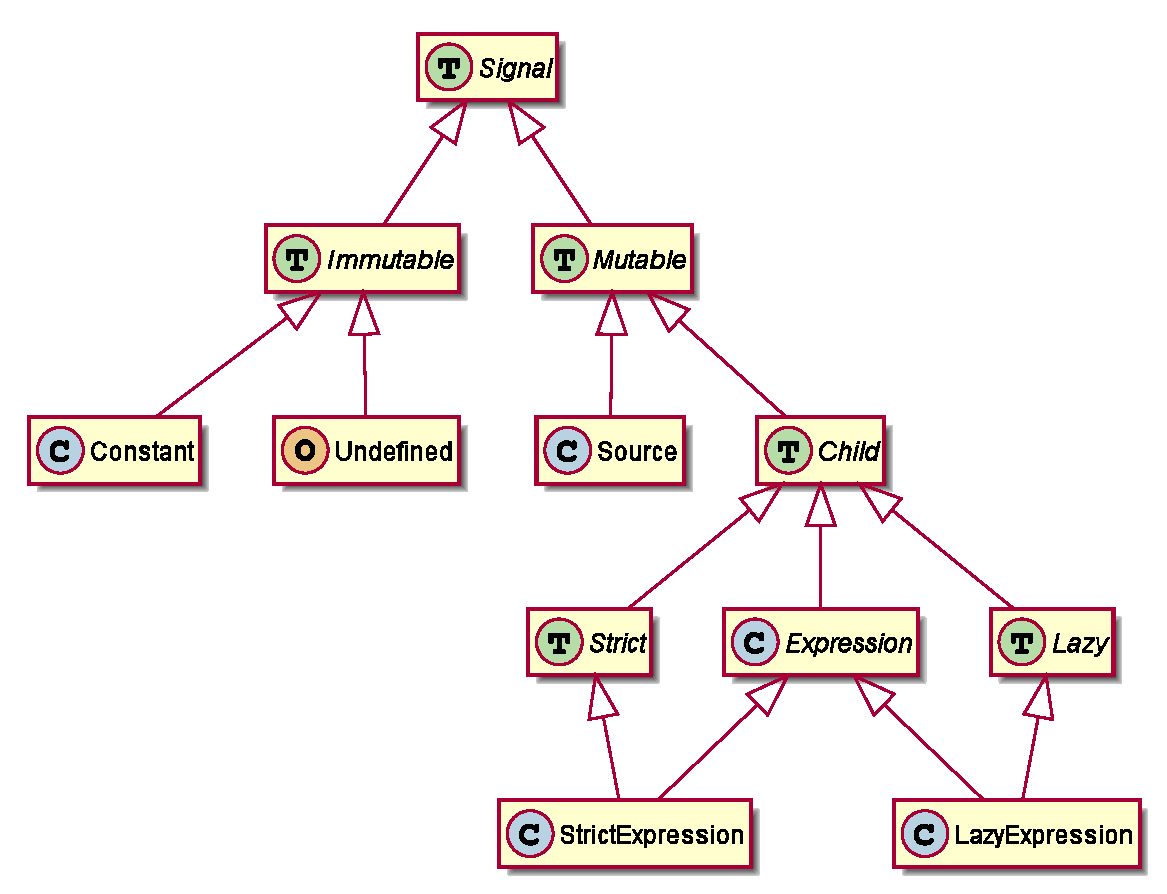
\includegraphics[width=10cm]{img/sig_hierarchy.eps}
	\caption{Hiérarchie des signaux}
	\label{fig:sig-hierarchy}
\end{figure}

L'implémentation des signaux est organisée sur la base du raffinement successif de la sémantique d'un signal. Chaque niveau laisse généralement un point de sa sémantique indéfini, sous la forme d'une méthode abstraite à implémenter par les sous-classes.

\begin{itemize}
	\item \texttt{Signal}: la vue la plus générale d'un signal, ce trait définit les méthodes de transformation et d'accès à l'état du signal. La fonction \texttt{def option: T} est indéfinie et doit retourner l'état courante du signal.
	\item \texttt{Immutable}: redéfinit \texttt{option} en \texttt{val} puisque l'état est immutable, mais laisse la valeur abstraite.
	\item \texttt{Constant}: définit \texttt{val option = Some(value)}
	\item \texttt{Undefined}: définit \texttt{val option = None}
	\item \texttt{Mutable}: déclare la méthode abstraite \texttt{def current: Option[T]}, représentant également l'état du signal mais dont le nom indique clairement la mutabilité du signal.
	
	Définit la méthode \texttt{option} en se basant sur \texttt{current} mais y ajoute la détection automatique des signaux enfants. De cette façon, toutes les méthodes de \texttt{Signal}, en utilisant directement ou indirectement \texttt{option}, obtiennent également les mécanismes de détection.
	
	\item \texttt{Source}: définit une variable interne pour stocker l'état de la source, implémente \texttt{current} sur la base de cette variable.
	
	Ajoute également les opérations de mutation explicites.
	
	\item \texttt{Child}: déclare la méthode abstraite \texttt{def generate: Option[T]}, appelée lorsque l'état du signal doit être calculé. Implémente \texttt{current} sur la base de \texttt{generate} et y ajoute le mécanisme de \emph{memoization}.
	
	Définit la méthode \texttt{def invalidate(): Unit} qui permet d'effacer l'état mémorisé du signal et d'invalider récursivement tous les signaux enfants. Cette méthode est en principe appelée par \texttt{Mutable}.
	
	\item \texttt{Lazy}: trait \emph{marqueur}, l'implémentation de \texttt{Child} utilise déjà la sémantique \emph{lazy} par défaut. Il n'y a donc rien à modifier.
	
	\item \texttt{Deferred}: surcharge la méthode \texttt{invalidate} définie par \texttt{Child} en insérant le signal dans la queue du contexte de mutation courant. De cette façon, ce signal sera recalculé de façon différée à la fermeture du contexte de mutation.
	
	\item \texttt{Expression}: implémente \texttt{generate} sur la base de l'expression passée en paramètre.
	
	\item \texttt{LazyExpr}: combine \texttt{Expression} avec \texttt{Lazy}
	\item \texttt{DeferredExpr}: combine \texttt{Expression} avec \texttt{Deferred}
\end{itemize}

Les classes \texttt{LazyExpr} et \texttt{DeferredExpr} sont privées. S'il est nécessaire dans le code utilisateur de déterminer la sémantique d'une expression, un \emph{pattern matching} sur les traits \texttt{Lazy} et \texttt{Deferred} peut être effectué. Il est également possible de tester si un signal est une expression constante avec l'opérateur \texttt{with}, sous la forme: \code{case e: Expression with Lazy}.

\subsection{Détection automatique des dépendances}

La détection automatique des dépendances des signaux et observateurs joue un rôle essentiel dans l'implémentation des signaux. Même à l'intérieur de la bibliothèque, aucune dépendance n'est déclarée explicitement et le détection automatique est utilisée.

L'élément clé de ce mécanisme est la classe \texttt{x.s.t.TracingContext}. Un contexte de traçage est un mécanisme très similaire à celui du contexte de mutation (§ \ref{sec:sig-mut-context}). Les deux sont construits sur la base du mécanisme de \texttt{DynamicVariable} présent dans la bibliothèque standard Scala.

Une opération de traçage est effectuée par un appel à la méthode
\begin{center}
	\code{def TracingContext.trace[T](expr: => T): (T, List[Mutable[_]])}
\end{center}
prenant en paramètre une expression arbitraire qui sera évaluée. La méthode retourne un couple de valeurs, dont le premier membre est le résultat de l'évaluation de l'expression et le second la liste de tous les signaux qui ont été accédés lors de cette évaluation.

Il convient de noter que seuls des signaux de type \texttt{Mutable[\_]} sont retournés. En effet, cette liste à pour but d'énumérer les dépendances de l'expression évaluée et ainsi permettre la mise en place des notifications de mises à jour. Un signal immutable ne changeant par définition jamais, il n'y a pas d'intérêt à le considérer comme une dépendance de l'expression.

La classe \texttt{DynamicVariable} est conçue pour représenter une variable dont la valeur et déterminée par portée dynamique plutôt que portée lexicale. C'est-à-dire que la valeur de la variable est déterminée dynamiquement selon la pile d'appel à l'exécution plutôt que par la structure du code source.

En pratique, il n'existe pas de portée dynamique en Scala, le concept est donc émulé en utilisant une pile locale au thread courant afin de stocker la valeur de la variable. La méthode
\begin{center}
	\code{def DynamicVariable[T].withValue[U](v: T)(expr: => U): U}
\end{center}
permet l'exécution d'un bloc de code arbitraire durant laquelle la méthode \texttt{DynamicVariable.value} retournera la valeur passée en paramètre. Chaque invocation de la méthode \texttt{withValue} ajoute un nouvel étage à la pile qui sera dépilé une fois l'évaluation terminée.

Dans le cas de \texttt{TracingContext}, un nouveau contexte est créé lors de l'appel à la méthode \texttt{trace} et placé dans une variable \texttt{DynamicVariable}. La seconde partie du système est implémentée dans la classe \texttt{Mutable}. Comme indiqué dans le détail de la hiérarchie des signaux (§ \ref{sec:sig-hierarchy}), cette classe implémente la méthode \emph{option} de \texttt{Signal} en y ajoutant le mécanisme de détection des dépendances.

Plus spécifiquement, chaque invocation de la méthode \texttt{option} d'un signal \texttt{Mutable} va appeler la méthode interne \texttt{TracingContext.record} afin d'enregistrer l'accès au signal dans le contexte courant. Déterminer le \emph{contexte courant} consiste en un simple accès à la variable \texttt{DynamicVariable} mentionnée précédemment.

Contrairement aux contextes de mutations, l'imbrication des contextes de traçage est significative. L'accès à un signal ne sera en effet enregistré que dans le contexte le plus récent, au sommet de la pile. Ceci découle de l'utilisation de contextes de traçage, en interne, par les signaux expression. 

L'objectif final est de limiter la liste des signaux retournés par la méthode \texttt{trace} aux dépendances directes de l'expression évaluée. Il n'est en effet pas intéressant de récupérer les dépendances \emph{transitives} d'un signal puisque les notification de mises à jour sont propagées récursivement jusqu'aux feuilles du graphe.

La figure \ref{fig:sig-nested-tracing} illustre une situation d'imbrication des contextes de traçage. L'évaluation du signal \emph{E} crée un nouveau contexte qui sera utilisé pour déterminer ses dépendances. Lors de l'évaluation du signal \emph{C}, un nouveau contexte est créé pour déterminer les dépendances de ce signal. Les signaux \emph{B} et \emph{A} forment ainsi des dépendances \emph{transitives} de \emph{E} et ne seront pas retournées dans la liste de signaux accédés par le signal \emph{E}, celle-ci se limitant aux signaux \emph{D} et \emph{C}.

\begin{figure}[h]
	\centering
	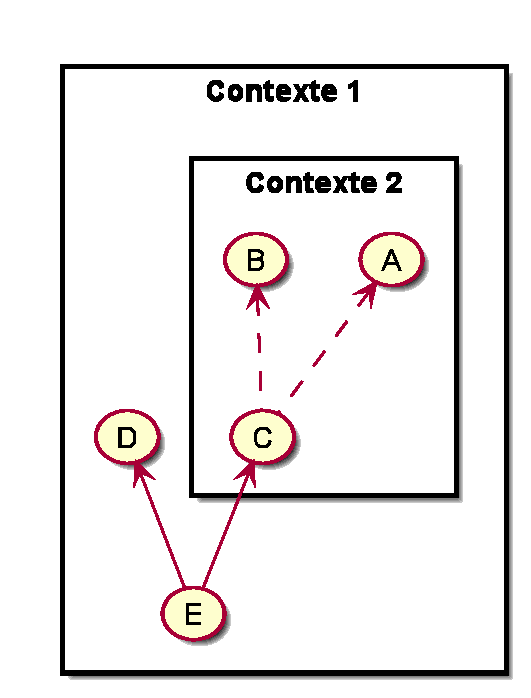
\includegraphics[width=5cm]{img/signals_nested_tracing.eps}
	\caption{Imbrication des contextes de traçage}
	\label{fig:sig-nested-tracing}
\end{figure}

Cette approche est une alternative à l'utilisation de paramètres implicites, tels qu'utilisés par la bibliothèque \emph{Scala.rx} \cite{scala.rx}. Les variables dynamiques forment un canal indépendant pour déterminer les relations de dépendance entre signaux et observateurs. Il n'est alors plus nécessaire de recourir à des macros compilateur pour transformer automatiquement l'expression fournie par l'utilisateur en fonction anonyme.

En contre-partie, la détection de dépendances est maintenant liée à la structure de la pile d'appels lors de l'accès aux signaux, ce qui implique une exécution synchrone des opérations. Les structures \emph{lazy} ou \emph{asynchrones} sont donc particulièrement problématiques puisqu'elles ne conservent pas la variable dynamique qui sera perdue dès la retour de l'appel synchrone. Dans un environnement \emph{single-threaded} tel que JavaScript, ceci n'est cependant pas un problème.

\subsection{Implémentation des opérateurs de transformation}

Lors de l'implémentation des opérateurs de transformation, deux approches ont été envisagées:
\begin{enumerate}
	\item Implémentation d'une sous-classe de \texttt{Signal} par transformation, par exemple des classes \texttt{Map}, \texttt{Fold}, etc. Cette approche est par exemple utilisée par la bibliothèque \emph{Bindings.scala} \cite{binding.scala}.
	\item Réutiliser le mécanisme des signaux expressions.
\end{enumerate}

La seconde approche a été choisie sur la base de la réutilisation de l'ensemble des mécanismes développés pour les signaux expression. Le seul élément à considérer est alors l'implémentation concrète de la transformation. Les détails annexes, tels que la sémantique d'évaluation ou la gestion des dépendances est obtenue de façon automatique.

Par exemple, la transformation \texttt{map} est déclarée simplement par
\begin{center}
	\code{def map[U](f: T => U): Signal[U] =}\\
	\code{Signal.define(option.map(f)) }
\end{center}
Ici, \texttt{option} fait référence à la méthode \texttt{Signal.option}. Le type de signal retourné par une transformation dépend du type de signal sur lequel elle est invoquée. Appliquer une transformation \texttt{map} sur un signal \texttt{Constant} retourne un nouveau signal \texttt{Constant}. Ceci résulte du fait que, lors du calcul de l'expression de définition de la transformation, aucun signal \texttt{Mutable} n'a été accédé. Le constructeur \texttt{Signal.define} retourne alors un signal de type \texttt{Constant} ce qui correspond au comportement attendu de la transformation.

Dans une version antérieure de l'implémentation des signaux, ces transformations étaient déclarées de façon abstraite dans l'interface \texttt{Signal} puis implémentées indépendamment dans les sous-classes \texttt{Mutable} et \texttt{Immutable}. Avec l'amélioration du constructeur \texttt{Signal.define}, prenant en compte les signaux accédés lors de la définition d'un nouveau signal, cette complexité a pu être éliminée et l'ensemble des signaux, mutables comme immutables, partagent maintenant une définition unique dans la classe parente \texttt{Signal}.

Un effet secondaire supplémentaire de cette implémentation est le support de fonctions de transformation impures. Référencer la valeur d'autres signaux dans une fonction passée aux opérateurs produira le résultat attendu. La figure \ref{fig:sig-map-pureness} illustre une telle situation où un même signal \texttt{Constant} est transformé en un nouveau signal \texttt{Constant} ou une \texttt{Expression} selon la pureté de la fonction passée en paramètre. Le support de ce style, bien que d'une élégance discutable, permet de réduire le risque de surprendre un utilisateur qui s'attendrait à pouvoir se servir de telles constructions.

\begin{figure}
	\begin{lstlisting}
val a: Constant[Int] = Constant(2)
val b: Signal[Int] = ...

val c = a.map(_ * 2)
// `c` est un signal `Constant[Int]`

val d = a.map(_ * b.value)
// `d` est un signal `Expression[Int]`
	\end{lstlisting}
	\caption{Exemple de transformation d'un signal constant en utilisant des fonctions pures ou impures}
	\label{fig:sig-map-pureness}
\end{figure}

\subsection{Modèle push, pull ou hybride}

Deux modes de fonctionnement sont généralement décrits pour des systèmes fonctionnels-réactifs: \emph{push} et \emph{pull}.

L'approche \emph{push} se base sur les changements apportés aux signaux sources pour recalculer tous les signaux enfants qui en dépendent. Dans l'approche \emph{pull}, c'est l'accès aux signaux enfants qui provoque le calcul des valeurs intermédiaires jusqu'aux signaux sources. Dans les deux cas, des opérations potentiellement inutiles ou redondantes sont effectuées.

L'approche mixte \emph{push-pull} se base sur une approche principalement \emph{pull} où l'accès à l'état d'un signal déclenche son évaluation, à laquelle vient s'ajouter un mécanisme de \emph{memoization} qui maintient l'état courant du signal après son calcul. L'invalidation de ces caches se fait ensuite selon une approche \emph{push}: un changement d'état des signaux sources est notifié à toutes les dépendances de façon récursive.

Dans le cadre de ce projet, l'approche \emph{pull} était tout simplement inutilisable. Lors de l'implémentation d'une interface utilisateur, les notifications de mises à jour proviennent des racines du graphe de signaux. L'interface ne connaît \emph{a priori} pas les moments opportuns à l'exécution d'un \emph{pull} pour se mettre à jour. L'approche \emph{push} est déjà plus adaptée, mais impose une mise à jour complète du graphe à chaque changement.

L'architecture proposée de l'application associe un graphe de signaux, représentant l'ensemble des données disponibles, avec un ensemble d'observateurs, correspondant aux données actuellement utilisées par l'interface. Il est courant qu'une partie de ce graphe soit inutilisée dans l'état courant de l'interface. Lorsque l'utilisateur navigue dans l'application, les observateurs des données qui ne sont plus visibles sont retirés tandis que de nouveaux sont attachés sur les données qui apparaissent à l'écran. Ainsi, les sections du graphe considérées actives changent dynamiquement en fonction des actions effectuées par l'utilisateur.

Le modèle hybride permet aux sections actives du graphe, celles dont les feuilles disposent d'observateurs, de se comporter effectivement de façon \emph{push} en étant recalculées dès lors que les données sources sont modifiées. À l'inverse, les sections inactives du graphe se comportent de façon \emph{pull}, n'étant pas recalculées inutilement tant qu'un observateur n'y aura pas été attaché ou leur état courant accédé de façon explicite.



\chapter{Framework web}

\section{Motivations}
\textit{Construction d'un framework d'interface web sur la base des signaux introduits précédemment.}

\textit{Développement spécifiquement pour Scala.js. Il existe de nombreux bindings par exemple pour React ou Angular en Scala.js, mais l'utilisation d'un framework conçu pour JavaScript en Scala.js n'est pas toujours l'expérience la plus agréable. Volonté de disposer d'une API conçue pour le langage Scala.}

\textit{Transition signaux -> component (via template et data binding)}

\section{À propos des standards Web Components}

L'implémentation de la partie web de Xuen dépend extensivement des mécanismes introduits par les spécifications \emph{Shadow DOM} \cite{w3c-shadowdom}, \emph{Custom Elements} \cite{w3c-custom-elements} et les spécifications annexes telles que \emph{CSS Scoping} \cite{w3c-css-scopings}.

Ces standards définissent des mécanismes permettant la définition de nouveaux éléments personnalisés, encapsulés et réutilisables. Ils définissent également comment l'encapsulation du composant est implémentée au niveau des styles CSS et des événements DOM. Ces mécanismes sont réutilisés avec le minimum d'abstraction lorsque cela est possible pour Xuen.

Définir un élément Xuen (§ \ref{sec:web-specs-element}) correspond à la définition d'un nouvel élément \emph{Custom Elements}: la classe produite est passée à la méthode native \texttt{define()} du navigateur tel que le serait une classe construite directement en JavaScript.

Les templates se basent sur \emph{Shadow DOM} comme mécanisme d'encapsulation. Ils peuvent ainsi réutiliser le concept de \texttt{<slot>} introduit par ce standard comme primitive de composition. L'encapsulation standard des événements et des styles s'applique également.

Ces concepts sont répartis entre une multitude de spécifications, provenant de différentes organisations et peuvent être difficiles à aborder de prime abord. Néanmoins, une connaissance des ces mécanismes peut se révéler très utile à la compréhension de l'implémentation et du fonctionnement de Xuen.

En guise d'introduction, le guide \emph{Shadow DOM v1: Self-Contained Web Components} \cite{google-shadowdom} rédigé par Google dans la série \emph{Web Fundamentals} est un bon tour d'horizon des mécanismes liés à Shadow DOM.

\section{Spécifications} \label{sec:web-specs}

\textit{L'architecture du framework web est encore à un stade très primitif.}

\subsubsection{Notation abrégée des packages}
Dans la suite de cette section, afin de réduire la longueur des noms des packages, une notation abrégée est utilisée à la place du nom complet d'une classe:
\begin{itemize}
	\item Le prefix \texttt{xuen} est abrégé en \texttt{x}.
	\item De façon similaire, le second niveau est abrégé en une seule lettre.
	\begin{itemize}
		\item \texttt{component} devient \texttt{c},
		\item \texttt{expression} devient \texttt{e},
		\item \texttt{template} devient \texttt{t},
		\item etc.
	\end{itemize}
\end{itemize}
Ainsi, par exemple, la classe \texttt{xuen.component.Element} est référencée par \texttt{x.c.Element}.

\subsection{Composant} \label{sec:web-usage-component}

Un composant est la brique essentiel de construction d'une application. Il correspond directement à une définition d'un \emph{custom element}. Une fois défini, un composant peut être instancié un nombre quelconque de fois, selon les besoins de l'application.

Un composant est défini à partir de:
\begin{itemize}
	\item Un sélecteur: correspondant à la balise HTML qui sera définie pour ce composant. Ce nom doit comporter un tiret (selon la spécification \emph{Custom Elements})
	\item Une implémentation: une sous-classe de \texttt{x.c.Element}, définissant le comportement des instances de ce composant
\end{itemize}
Optionnellement, un composant peut également posséder:
\begin{itemize}
	\item Un template: une structure HTML pouvant contenir des expressions de \emph{data-binding} avec des données réactives sous la forme de signaux, ce template sera matérialisé pour chaque instance du composant 
	\item Une feuille de styles: pouvant être utilisée pour définir l'apparence visuelle du composant
	\item Une liste de dépendances: une liste d'autres composants devant être chargés avant ce composant, cette liste correspond à d'autres composants utilisés dans le template de ce composant.
\end{itemize}

\subsubsection{Déclaration}
En pratique, un composant est créé en déclarant un \texttt{object} qui étend la classe \texttt{x.c.Component}. La classe correspondant à l'implémentation du composant est généralement déclarée simultanément avec le même nom, formant ainsi une paire (classe, objet compagnon) fréquent en Scala.

\begin{lstlisting}
import xuen.component._

class HelloWorld extends Element(HelloWorld)

object HelloWorld extends Component[HelloWorld](
	selector = "hello-world",
	template = html"""
		Hello, world!
	""",
	stylesheet = css"""
		:host { color: blue; }
	"""
)
\end{lstlisting}

Ce court exemple illustre déjà la plupart des concepts utilisés dans la construction de composants Xuen.

\subsubsection{Interpolateurs \texttt{html} et \texttt{css}}

Lors de la définition du template et de la feuille de style d'un composant, les interpolateurs \texttt{html} et \texttt{css} sont généralement utilisés. Ils sont une façon simple d'obtenir les objets de type \texttt{Template} et \texttt{Stylesheet} attendu par le constructeur de \texttt{Component} à partir de code source HTML ou CSS.

Ces interpolateurs sont définis par la classe \texttt{x.c.Interpolations}. En Scala, l'implémentation de tels interpolateurs repose sur l'utilisation de conversions implicites qui ne sont généralement pas identifiées automatiquement par l'IDE. Il est ainsi nécessaire d'importer cette classe manuellement afin de les utiliser. Alternativement, il est possible d'importer l'ensemble du package \texttt{xuen.component} en utilisant une importation \texttt{wildcard}.
\begin{lstlisting}
import xuen.component._
\end{lstlisting}
Cette méthode est généralement préférée à l'importation explicite.

Le nom d'interpolateur est trompeur: contrairement à l'interpolateur \texttt{s} de la bibliothèque Scala, \texttt{html} et \texttt{css} ne supporte pas l'insertion de fragments à l'aide du symbole spécial \texttt{\$}. Ils sont cependant une façon concise d'appliquer un traitement à une chaîne de caractères, en l'occurrence la transformation en instance de \texttt{Template} ou \texttt{Stylesheet}. Ils sont également l'occasion pour l'IDE d'identifier le langage utilisé dans la chaîne de caractères et ainsi offrir une coloration syntaxique et une auto-complétion appropriée.

Dans le cas d'IntelliJ IDEA, il est possible d'associer des langages arbitraires avec un interpolateur. Il est ainsi possible d'associer l'interpolateur \texttt{html} avec le langage HTML, de même pour \texttt{css} avec CSS. Dès lors, le code du template ou de la feuille de style sera correctement traité comme HTML ou CSS dans l'éditeur.

\subsubsection{Enregistrement et instantiation}

L'enregistrement du composant en tant que \emph{custom element} au niveau du navigateur se fait automatiquement lors de la construction de l'objet singleton \texttt{x.c.Component} de ce composant.

En Scala, la construction d'un \texttt{object} est différée jusqu'à la première référence de cet élément dans le code source, de façon similaire à l'initialisation d'une \texttt{lazy val}. La simple présence de la définition dans le code source n'est donc pas suffisante pour que ce composant soit enregistré. La méthode par laquelle le composant est instancié est alors importante.

Un composant peut être instancié de 4 façons différentes:
\begin{enumerate}
	\item Par l'utilisation du constructeur de son implémentation:
	\begin{lstlisting}
val element = new HelloWorld
	\end{lstlisting}
	\item En utilisant la méthode \texttt{instantiate} de \texttt{Component}:
	\begin{lstlisting}
val element = HelloWorld.instantiate()
	\end{lstlisting}
	\item En utilisant la méthode \texttt{createElement} de \texttt{Document}:
	\begin{lstlisting}
val element = dom.document.createElement("hello-world")
	\end{lstlisting}
	\item Implicitement par le parser HTML:
	\begin{lstlisting}
val div = dom.document.createElement("div")
div.innerHTML = "<hello-world></hello-world>"
	\end{lstlisting}
\end{enumerate}

Dans les deux premiers cas, l'objet \texttt{Component} est référencé directement ou indirectement et il n'est pas nécessaire de se préoccuper de l'enregistrement. Ce sont les méthodes préférées lorsque le composant est instancié par le code du développeur et non le navigateur lui-même.

Les deux autre méthodes se basent sur l'API native du navigateur et ne référencent à aucun moment l'objet \texttt{Component}. Ces méthodes n'enregistrent ainsi pas le composant au niveau du navigateur. Dans une telle situation, la fonction \texttt{Component.register} peut être utilisée pour forcer une référence vers l'objet \texttt{Component}. Un nombre arbitraire de composant peuvent être passés à \texttt{register}.
\begin{lstlisting}
Component.register(HelloWorld, AnotherComponent, ...)
\end{lstlisting}

Dans le cas des composants utilisés dans le template d'un autre composant, ces composants doivent être explicitement spécifiés dans la liste de dépendances du composant de premier niveau. Ainsi, référencer l'objet \texttt{Component} de niveau supérieur référencera également tous les composants des niveaux inférieurs et les enregistrement seront correctement effectués.
\begin{lstlisting}
object HelloWorld extends Component[HelloWorld](
	...,
	dependencies = List(One, Two, Three)
)
\end{lstlisting}

\subsection{Element} \label{sec:web-specs-element}

La définition du comportement d'un composant se fait par la définition d'une sous-classe de \texttt{x.c.Element} qui est ensuite passée au constructeur de \texttt{Component} (§ \ref{sec:web-usage-component}). Chaque instance du composant sera alors une instance de cette classe.

Un élément hérite de tous les éléments nécessaires à la définition d'un comportement de composant par le biais de la classe \texttt{x.c.Element}. Le seul paramètre restant à spécifier est le composant qui est implémenté par cet élément, ce qui est effectué par la paramètre passé au constructeur de \texttt{Element}.
\begin{lstlisting}
class HelloWorld extends Element(component = HelloWorld)
\end{lstlisting}

La déclaration ci-dessus est donc suffisante pour la définition d'un comportement de composant valide. La classe \texttt{Element} offre de nombreux outils aux instances de ses sous-classes.

\subsubsection{Interface \texttt{HTMLElement}}
\texttt{Element} hérite de l'interface \texttt{HTMLElement}, définie par le navigateur et les standards web. Cette interface hérite à son tour d'un ensemble d'autres interfaces tels que \texttt{dom.Element}\footnote{La spécification DOM défini également une interface \texttt{Element}, à distinguer de la classe abstraite \texttt{xuen.component.Element} qui est une implémentation spécifique de cette interface. En pratique, l'interface \texttt{x.c.Element} est rarement utilisée par le code utilisateur, et l'interface DOM est généralement utilisée en tant que \texttt{dom.Element} en Scala.js}, \texttt{dom.Node}, \texttt{EventTarget}.

Une instance de \texttt{Element} possède donc les méthodes et attributs usuels des éléments HTML, tel que par exemple \texttt{style}, \texttt{parentNode}, \texttt{querySelector} ou \texttt{addEventListener}. C'est aussi un argument valide pour les méthodes de manipulation du DOM tel que \texttt{appendChild} ou \texttt{replaceChild}.

\subsubsection{ShadowRoot}
Xuen se base sur les mécanismes du \emph{Shadow DOM} pour implémenter templates et feuilles de styles. Chaque instance d'un composant est ainsi associée à un sous-arbre Shadow DOM, accessible depuis l'attribut \texttt{shadow} définie par la classe \texttt{Element}.

Cet attribut est similaire à l'attribut \texttt{shadowRoot} définie par la spécification Shadow DOM à la différence que \texttt{shadow} est garanti d'être non-nul. Un sous-arbre Shadow DOM est automatiquement construit lors de l'accès à l'attribut si celui-ci n'existe pas. Un sous-arbre Shadow DOM est également automatiquement construit si le composant a défini un template ou une feuille de style et sera initialement peuplé par les éléments correspondants.

Il est généralement déconseillé de manipuler le sous-arbre Shadow DOM manuellement. Ceci est en général effectué de façon déclarative à partir du template. Il peut cependant être nécessaire d'accéder à l'instance d'un élément présent dans le sous arbre à partir de l'implémentation du composant. Dans une telle situation \texttt{querySelector} peut être utilisé à partir de \texttt{shadow} pour accéder aux éléments du sous-arbre.

\begin{lstlisting}
class HelloWorld extends Element(HelloWorld) {
	private val span = shadow.querySelector("span")
	span.addEventListener("click", ...)
}

object HelloWorld extends Component[HelloWorld](
	selector = "hello-world",
	template = html"""Hello, <span>world</span>!"""
)
\end{lstlisting}

À noter que, conformément à la spécification Shadow DOM, invoquer la méthode \texttt{querySelector} directement sur l'instance \texttt{Element} ne permet pas d'accéder aux éléments du sous-arbre Shadow DOM, uniquement aux enfants hors du sous-arbre caché, appelé \emph{light DOM}.

\begin{lstlisting}
// Instancié à partir de :
// <hello-world><span>a</span></hello-world>

class HelloWorld extends Element(HelloWorld) {
	private val a = this.querySelector("span")
	private val b = this.shadow.querySelector("span")
	assert(a.textContent == "a")
	assert(b.textContent == "b")
}

object HelloWorld extends Component[HelloWorld](
	selector = "hello-world",
	template = html"""<span>b</span>"""
)
\end{lstlisting}

\subsubsection{Attributs}
Les attributs jouent un rôle similaire aux arguments de constructeur en HTML, ils sont un mécanisme permettant de passer des paramètres à un élément afin de configurer son comportement.

Un élément Xuen peut définir un ensemble de paramètre auxquels il souhaite avoir accès sous forme d'un signal \texttt{Source}. La valeur de l'attribut sera reflétée dans le signal correspondant. Cette association est \emph{live}, c'est à dire que l'attribut sera automatiquement observé et la valeur du signal sera mise à jour si un événement externe venait à modifier sa valeur. Inversement, un changement de la valeur de la source entraînera automatiquement une mise à jour de l'attribut HTML correspondant.

Un \emph{binding} d'attribut est déclaré en utilisant la méthode \texttt{attribute[T]}, produisant un \texttt{Source} de type \texttt{T} pour l'attribut. Le nom de l'attribut est automatiquement déterminé en fonction du nom de la variable à laquelle cette source est associée.

\begin{lstlisting}
class HelloWorld extends Element(HelloWorld) {
	val foo = attribute[String]
	// Association avec l'attribute `foo`
}
\end{lstlisting}

Si la détection automatique ne parvient pas à identifier automatiquement le nom de l'attribut en question, une erreur sera générée à la compilation. Il est alors possible de spécifier explicitement le nom de l'attribut. Ceci permet également d'associer un nom différent à la source et à l'attribut manipulé.

\begin{lstlisting}
class HelloWorld extends Element(HelloWorld) {
	val bar = attribute[String]("foo")
}
\end{lstlisting}

La valeur d'un attribut d'un élément HTML est toujours une chaîne de caractères. Un \emph{binding} d'attribut effectue automatiquement une sérialisation ou désérialisation entre la valeur effective de l'attribut de type \texttt{String} et le type \texttt{T} utilisé par le signal.

Cette opération nécessite qu'une instance du trait \texttt{x.c.AttributeFormat[T]} soit implicitement disponible pour le type \texttt{T} en question. Par défaut, les types \texttt{String}, \texttt{Boolean}, \texttt{Char}, \texttt{Byte}, \texttt{Short}, \texttt{Int}, \texttt{Long}, \texttt{Float} et \texttt{Double} peuvent être utilisés pour un attribut.

\subsubsection{Propriétés}
Les propriétés sont une alternative aux attributs qui ne dépendent pas de \texttt{AttributFormat} et peuvent donc être utilisés pour passer n'importe quel type de paramètre à un élément Xuen. 

\begin{lstlisting}
class HelloWorld extends Element(HelloWorld) {
	val foo = property[Map[Int, String]]
}
\end{lstlisting}

En pratique, une déclaration \texttt{property[T]} correspond à la construction d'une \texttt{Source.undefined[T]}. Cependant, l'usage de \texttt{property} souligne l'usage attendu de la source en tant que paramètre de l'élément.

\subsubsection{Événements personnalisés}

\textit{Méthodes simplifiée pour le traitement d'événement personnalisés dans un Element.}

\subsubsection{Événements \texttt{xuen:connected} et \texttt{xuen:disconnected}}

\textit{Custom events lors de la connexion / déconnexion d'un élément}

\subsection{Template}

Un template est une structure de noeuds DOM qui sont automatiquement insérés dans le sous-arbre Shadow DOM d'un composant lorsque celui-ci est instancié. Cette structure est généralement définie à partir du code source HTML correspondant et l'interpolateur \texttt{html}, en paramètre au constructeur de \texttt{Component}.

Cette structure est \emph{compilée} lors de la création de l'objet correspondant \texttt{Template}. Le compilateur va ainsi parcourir récursivement la structure originale afin d'identifier des annotations de \emph{data-binding} associant des comportements particuliers à certains noeuds de l'arbre.

Ces annotations sont fortement inspirées de la syntaxe utilisée par le framework \emph{Angular 2} et prennent la forme d'attributs particuliers placés sur les éléments du template. La comportement exact de ces annotations est spécifié par l'\emph{expression} utilisée comme valeur de l'attribut. La section \ref{sec:web-usage-expr} détail spécifiquement la syntaxe des expressions. Cette section se concentre sur les annotations disponibles.

\subsubsection{Interpolation}
Les noeuds \texttt{Text} et les attributs d'éléments présents dans le template peuvent contenir des marqueurs d'interpolation \texttt{\{\{ \}\}}. L'expression contenue dans la double-paire d'accolade sera évaluée puis convertie en \texttt{String} avant d'être insérée à la place du marqueur dans le texte final.

\begin{lstlisting}[language=HTML]
<div>2 + 2 = {{ 2 + 2 }}</div>
--> <div>2 + 2 = 4</div>

<canvas width="720" height="{{9/16 * 720}}"></canvas>
--> <canvas width="720" height="405"></canvas>
\end{lstlisting}

Une expression d'interpolation ne peut jamais échouer, les cas de valeurs \texttt{null} et \texttt{undefined} sont explicitement gérés en retournant le texte correspondant. Dans tous les autres cas, la méthode \texttt{toString} est utilisée pour produire la valeur finale.

Il n'est pas possible de placer une interpolation dans un attribut dont le contenu est déjà interprété comme une expression. C'est par exemple le cas des attributs qui sont des annotations de \emph{data-binding}. Il n'est pas non plus possible d'emboîter une interpolation dans une autre.

Il est cependant autorisé de placer une interpolation dans un commentaire HTML comme utilitaire de développement.

\subsubsection{Annotation d'identifiant}
Un attribut dont le nom débute par \texttt{\#} est traité comme une annotation d'identifiant, spécifiant la valeur de l'attribut \texttt{id} de l'élément. Cette simple annotation est principalement un sucre syntaxique et la valeur de l'attribut, si elle est spécifiée, est ignorée.

\begin{lstlisting}[language=HTML]
<div #foo></div>
--> <div id="foo"></div>
\end{lstlisting}

\subsubsection{Annotation de classe}
Un attribut dont le nom commence par \texttt{.} est traité comme une annotation de classe. Si aucune valeur n'est fournie pour cet attribut, la classe est inconditionnellement ajoutée aux classes de l'élément.

Si une valeur est fournie pour cet attribut, celle-ci évaluée en tant qu'expression booléenne. Si la valeur évaluée est \texttt{true}, la classe est ajoutée à la liste de classes de l'élément. Dans le contraire, la classe est retirée de l'élément. Si cette expression utilise des signaux, ce comportement est dynamique et la classe correspondante sera ajoutée ou retirée au fil du temps.

\begin{lstlisting}[language=HTML]
<div .foo .bar="true" .baz="false"></div>
--> <div class="foo bar"></div>
\end{lstlisting}

\subsubsection{Annotation de propriété}
Un attribut dont le nom commence par \texttt{[} et se termine par \texttt{]} est traité comme une annotation d'attribut.

La valeur de l'attribut est évaluée en tant qu'expression et la valeur obtenue est utilisée pour mettre à jour la propriété correspondante de l'élément. Si cette propriété est une \texttt{Source}, la valeur de la source est modifiée à la place.

\begin{lstlisting}[language=HTML]
<input type="text" [value]="2 + 2">
--> <input type="text"> == $0
--> $0.value == "4"
\end{lstlisting}

Il est important de souligner que ce type d'annotation n'affecte pas les \emph{attributs} de l'élément mais bien les \emph{propriétés} de l'objet JavaScript correspondant. C'est pourquoi dans l'exemple ci-dessus il n'y a pas d'attribut \texttt{value} présent sur l'élément \texttt{<input>}, mais \texttt{\$0.value} retourne effectivement la chaîne de caractères \texttt{"4"}\footnote{La notation \texttt{\$0} est inspirée de l'inspecteur web de Google Chrome, dans lequel la variable \texttt{\$0} fait référence à l'élément actuellement sélectionner dans l'inspecteur DOM.}.

Si aucune valeur n'est fournie pour l'annotation de propriété, la nom de la propriété est utilisée comme expression. Ainsi, une annotation \texttt{[foo]} est traitée en tant que \texttt{[foo]="foo"}, offrant ainsi une syntaxe raccourcie dans le cas où une propriété d'un élément parent est passée tel quel à une propriété du même nom dans un élément enfant.

\subsubsection{Annotation d'événement}

Un attribut dont le nom commence par \texttt{(} et se termine par \texttt{)} est traité comme une annotation d'événement.

La valeur de l'attribut sera évaluée à chaque fois que l'événement correspondant sera \emph{dispatché} à partir de l'élément. À l'intérieur de cette expression, la variable \texttt{event} fait référence à l'instance de l'événement émis. Il est interdit de ne pas spécifier de valeur pour une annotation d'événement.

\begin{lstlisting}[language=HTML]
<input type="text" (input)="doSomethingWith(event.target.value)">
\end{lstlisting}

Les événements sont écoutés sur l'élément annoté, et du point de vue de l'élément parent. En d'autre termes, le gestionnaire d'événement est attaché à l'élément lui-même, il n'y a donc pas besoin que l'élément se propage dans l'arbre DOM pour être reçu. En revanche, si l'élément provient du sous-arbre Shadow DOM de l'élément, il est possible qu'il ne traverse pas la barrière du Shadow DOM et soit ainsi invisible à partir de l'élément parent.

Un certains nombre d'événements traversent naturellement la barrière du Shadow DOM, c'est la cas par exemple de \texttt{click}, \texttt{input} ou \texttt{mousemove}. D'autres, comme par exemple tous les événements personnalisés, sont par défaut encapsulés dans le sous-arbre et invisibles de l'extérieur de l'élément. Un tel événement ne pourra être capturé par cette annotation. Dans le cas d'un événement personnalisé, il est nécessaire que le flag \texttt{composed} soit défini à \texttt{true} lors de la création de l'événement.

\subsubsection{Transformation \texttt{*if}}
Une transformation est une annotation qui modifie dynamiquement la structure du DOM à partir d'expressions.

La transformation \texttt{*if} évalue sa valeur en tant qu'expression booléenne. Si la valeur obtenue est \texttt{true}, l'élément est inséré dans l'arbre DOM. Si la valeur est \texttt{false}, l'élément est retiré de l'arbre et un commentaire est inséré à la place en tant que \emph{placeholder}.

\begin{lstlisting}[language=HTML]
<div> <div *if="true"></div> </div>
--> <div> <div></div> </div>

<div> <div *if="false"></div> </div>
--> <div> <!-- *if false --> </div>
\end{lstlisting}

\subsubsection{Transformation \texttt{*for}}
La valeur de la transformation \texttt{*for} doit être un \texttt{énumérateur}, une expression particulière définissant les différentes propriétés de l'itération. Pour chaque élément de l'énumérateur, l'élément sera dupliqué et inséré dans l'arbre DOM.

À l'intérieur d'un élément annoté avec \texttt{*for}, les variables déclarées par l'énumérateur sont accessibles et correspondent à la valeur courante de l'itération. Il est également possible d'utiliser ces variables pour d'autres annotations présentes sur l'élément, les transformations étant appliquées avant les annotations.

\begin{lstlisting}[language=HTML]
<ul> <li *for="i of [1, 2, 3]">{{i}}</li> </ul>
--> <ul> <li>1</li> <li>2</li> <li>3</li> </ul>
\end{lstlisting}

\subsubsection{Précédence des transformations}
Si les transformation \texttt{*if} et \texttt{*for} sont simultanément présentes sur un élément, la transformation \texttt{*if} est appliquée en premier, suivi de la transformation \texttt{*for}.

L'objectif est d'offrir un mécanisme permettant la désactivation conditionnelle de l'ensemble de l'itération, en traitant \texttt{*if} avant \texttt{*for}, plutôt que l'élision d'un élément particulier de l'itération, ce qui se produirait si \texttt{*for} était évalué avant \texttt{*if}. En effet la clause de filtrage \texttt{if} de l'énumérateur offre déjà ce mécanisme.

\subsubsection{Utilisation combinée des transformations avec \texttt{<template>}}
Du fait de la syntaxe du langage HTML, il n'est possible d'appliquer une annotation que sur un élément, et non un noeud DOM quelconque. Il n'est par exemple pas possible d'annoter un noeud \texttt{Text}.

Dans le cas des annotations basiques, cela n'a généralement pas d'importance, un noeud \texttt{Text} ne possède de toutes façons pas d'attribut \texttt{id}, \texttt{class} ou de propriétés particulières. Il n'émet pas non plus d'événements. Cependant, dans le cas des annotations de transformations, l'impossibilité d'annoter un noeud \texttt{Text} peut se révéler gênant.

\begin{lstlisting}[language=HTML]
<div><span>...</span> ??*if="..."??text <span>...</span></div>
--> Nothing to put the `*if` on ?!
\end{lstlisting}

Au autre situation problématique est l'annotation simultanée de plusieurs éléments. Comment faire lorsque une transformation \texttt{*for} doit produire deux éléments DOM pour chaque élément de l'itération ? Dans l'exemple ci-dessous, chaque \emph{checkbox} est associée à un label.

\begin{lstlisting}[language=HTML]
<input *for="i of [1, 2]" type="checkbox" [value]="i">
<span *for="i of [1, 2]">{{i}}</span>
\end{lstlisting}

Cet exemple produit une liste de 3 \emph{checkboxes} puis 3 labels, certainement pas le résultat escompté.

Une solution serait d'encapsuler les noeuds à annoter dans une élément neutre tel que \texttt{<div>} ou \texttt{<span>} et d'annoter cet élément. Cette solution est relativement simple et est généralement la méthode préférée dans ce genre de situation.

Cependant, l'ajout d'un élément supplémentaire peut avoir des effets secondaires indésirables, par exemple au niveau des sélecteurs CSS. Dans le cas d'une itération, ceci n'est pas toujours possible. Dans ces situations, il est possible d'utiliser un élément \texttt{<template>} afin d'encapsuler un nombre quelconque de sous-noeuds DOM.

\begin{lstlisting}[language=HTML]
<template *for="i of [1, 2]">
	<input type="checkbox" [value]="i">
	<span>{{i}}</span>
</template>
\end{lstlisting}

Lorsqu'une transformation est appliquée sur un élément \texttt{<template>}, cet élément est supprimé du sous-arbre DOM produit par la transformation et seul son contenu est inséré. Il se substitue ainsi à l'élément encapsulant mentionné précédemment et disparait totalement lors de l'application de la transformation.

\subsection{Expressions} \label{sec:web-usage-expr}
Les expressions sont à la base des comportements dynamiques dans les templates Xuen. Elles sont fortement inspirées de la syntaxe de JavaScript et suivent en grande partie la sémantique de celui-ci.

Les expressions sont conçues pour être utilisées en combinaison avec les signaux Xuen. Le résultat de l'évaluation d'une expression est transformé en \texttt{Signal}, permettant ainsi de profiter du mécanisme de propagation des changements implémentés dans les signaux. Lorsqu'un signal référencé dans une expression change, la valeur de l'expression est recalculée et le template mis à jour en conséquence.

À l'intérieur même d'une expression, les signaux accédés sont décomposés par l'interpréteur. Si l'interpréteur rencontre un fragment d'expression produisant une valeur de type \texttt{Signal[T]}, cette valeur sera transformée en simple \texttt{T} en invoquant la méthode \texttt{value} du signal. Ce processus est récursif, une valeur de type \texttt{Signal[Signal[T]]} sera également extraite en une valeur \texttt{T}. Si un signal indéfini est rencontré, la valeur \texttt{undefined} est utilisée à la place. L'évaluation de l'expression continue alors avec la nouvelle valeur.

Il n'est donc pas nécessaire lors de la construction d'une expression de se soucier de l'encapsulation d'une valeur dans un signal puisque celui-ci sera automatiquement retiré par l'interpréteur.

\begin{figure}[h]
	\begin{lstlisting}
class HelloWorld extends Element(HelloWorld) {
	val name = attribute[String]
	// `name` est une `Source[String]` une sous-classe de `Signal[String]`
}

object HelloWorld extends Component[HelloWorld](
	selector = "hello-world",
	template = html"""
		Hello, {{name}}!
		<!-- Dans une expression, `name` est traité comme une simple valeur `String` -->
	"""
)

// Utilisation:
<hello-world name="Bastien"></hello-world>
	\end{lstlisting}
	\caption{Exemple illustrant l'extraction automatique des valeurs \texttt{Signal} lors de l'évaluation d'une expression}
\end{figure}

\subsubsection{Contexte d'évaluation}
Une expression est toujours évaluée par rapport à un contexte spécifique. Ce contexte défini le monde extérieur autour de l'expression. Il est pas exemple utilisé lorsque l'expression fait référence à des variables ou des fonctions. Dans ce cas, le contexte est invoqué pour obtenir la valeur de cette variable.

Dans la plupart des cas, le contexte d'une expression sera l'\texttt{Element} auquel le template est associé. Les variables et les fonctions invoquées correspondent respectivement aux propriétés et méthodes de l'objet \texttt{Element}.

\begin{lstlisting}
class HelloWorld extends Element(HelloWorld) {
	val foo = 2
	def bar(v: Int): Int = v * 3
}

<div>{{ foo + bar(5) }}</div>
--> <div>17</div>
\end{lstlisting}

Certaines constructions, par exemple une transformation \texttt{*for} ou une annotation d'événement, peuvent introduire des contextes \emph{enfants}. Ces contextes sont comparables au concept de \emph{scope} d'un langage de programmation. Les propriétés présentes sur le contexte enfant sont disponibles en plus des propriétés du contexte parent. Dans le cas où une propriété est présente à la fois dans le contexte parent et le contexte enfant, la propriété du contexte enfant masque celle du contexte parent (\emph{shadowing}).

\begin{lstlisting}
class HelloWorld extends Element(HelloWorld) {
	val foo = List(3, 5)
	val i = 8
	val j = 13
}

<div>
	<span>{{i + j}}</span>
	<span *for="i of foo">{{i + j}}</span>
</div>
--> <span>21</span> <span>16</span> <span>18</span>
\end{lstlisting}

\subsubsection{Opérateur d'accès protégé \texttt{?.}}
L'opérateur \texttt{?.} est similaire à l'usage à l'opérateur simple \texttt{.}: il permet d'accéder à une propriété ou une méthode de l'expression à sa gauche et prend un identifier à sa droite pour identifier la propriété accédée.

En revanche, lorsque l'expression à gauche de l'opérateur \texttt{.} est \texttt{undefined}, tenter de l'indexer avec l'opérateur \texttt{.} provoque une erreur. Ceci est utile en phase de développement pour identifier les situations où une référence qui ne devrait pas être indéfinie l'est tout de même.

Dans le cas où il est normale que le membre de gauche puisse être \texttt{undefined}, l'usage de l'opérateur protégé \texttt{?.} ne provoque pas d'erreur et retourne simplement \texttt{undefined} à son tour, permettant ainsi de le chaîner autant de fois que nécessaire. Si la référence indexée est définie, l'opérateur \texttt{?.} se comporte de façon identique à l'opérateur \texttt{.} classique.

\subsection{Feuille de styles}
La feuille de styles d'un composant est un simple fragment de code CSS qui sera injecté dans le sous-arbre Shadow DOM d'un composant. Aucun traitement particulier n'est appliqué au code source CSS.

La feuille de styles est injectée sous la forme d'un élément \texttt{<style>} contentant les définitions CSS. Puisque cet élément est placé dans un sous-arbre DOM, la portée de ses sélecteurs est limitée à ce sous-arbre. Il n'y a donc pas de conflits au niveau des identifiant des éléments du template (attribut \texttt{id}) ou du nom des classes, conduisant à des sélecteur extrêmement simples et concis.

Spécifiquement l'élément \texttt{<style>} est inséré en tant que dernier enfant du sous-arbre Shadow DOM. Ce qui a pour implication que le dernier élément du template ne vérifie pas le sélecteur \texttt{:last-child}, puisque l'élément \texttt{<style>} est en pratique le dernier élément du template. En revanche, le sélecteur \texttt{:first-child} identifie correctement le premier élément dans le template. Si l'usage du sélecteur \texttt{:last-child} s'impose, il est possible d'envelopper le template dans un élément \emph{wrapper} et ainsi ignorer la présence de l'élément \texttt{<style>} en tant que dernier fils du sous-arbre.

Il est possible de faire référence à l'élément hôte lui même, c'est à dire l'élément possédant la racine du sous-arbre Shadow DOM, avec le sélecteur \texttt{:host}. La version fonctionnelle de ce sélecteur (\texttt{:host(selector)}) permet de faire référence à l'élément hôte uniquement si celui-ci vérifie également le sélecteur passé en paramètre.

L'élément sélectionné par le sélecteur \texttt{:host} correspond à l'élément personnalisé lui-même, qui est également accessible en dehors du sous-arbre Shadow DOM. Dans le cas où une propriété CSS est définie à la fois à l'intérieur (par la feuille de styles de l'élément lui-même) et à l'extérieur du sous-arbre Shadow DOM (par une feuille de styles dans le contexte parent), la définition extérieur s'applique et la définition intérieur est ignorée. Par exemple, la marge interne d'un élément \texttt{<hello-world>} dont la feuille de styles contiendrait \texttt{:host \{ padding: 12px; \}} pourrait être modifiée en spécifiant: \texttt{hello-world \{ padding: 0px; \}} dans la feuille de styles de l'élément parent (ou du document).

Ces sélecteurs ne sont pas une spécificité de Xuen, ils font partie de la spécification \emph{CSS Scoping} des standards web. Puisque Xuen se base sur l'implémentation standard des \emph{Web Components} pour ses propres composants, il est possible de profiter des standards annexes développés pour \emph{Web Components} lorsque cela est applicable.

\subsubsection{Variables CSS}
Le mécanisme de variables CSS est également un standard web qui est à présent implémenté dans la quasi-totalité des navigateurs modernes. En pratique le support des variables CSS est plus répandu que le support de \emph{Shadow DOM} et \emph{Custom Elements}, elles peuvent donc être considérée comme utilisables dans ce projet.

Une variable CSS prend la forme d'une propriété personnalisée dont le nom débute par deux tiret \texttt{--}. Par exemple, la déclaration \texttt{--foo: 2} défini une variable \texttt{--foo} dont la valeur est \texttt{2}.

Le nom de \emph{variable} est trompeur. En pratique, ces constructions se comportent plus comme une constante, qui est propagée entre les éléments par le mécanisme de cascade classique de CSS. Cette valeur peut alors être redéfinie et la nouvelle valeur sera effective pour le reste de la cascade.

Ceci peut être comparé à la valeur de la propriété \texttt{font-size} qui est appliquée par cascade à tous les sous-élément de l'élément auquel elle est appliquée, et qui peut être écrasée par la définition d'une nouvelle propriété \texttt{font-size} sur l'un de ces sous-éléments.

La valeur d'une variable CSS est accédée par la fonction \texttt{var()} prenant le nom de la variable en paramètre et optionnellement une valeur par défaut. Par exemple,
\begin{lstlisting}[language=HTML]
body {
	--bg-color: blue;
}

div {
	background-color: var(--bg-color, red);
}
\end{lstlisting}

Les variables CSS sont la méthodes préférée pour paramétrer l'apparence d'un élément personnalisé. La liste des variables CSS utilisée par un élément sont ainsi une part intégrale de l'interface publique de l'élément.

\subsection{Service}

\subsection{Router}

\section{Solutions existantes}

\subsection{Bindings.scala et Monadic-HTML}

\emph{Bindings.scala} \cite{binding.scala} et \emph{Monadic-HTML} \cite{monadic-html} sont deux exemples d'implémentation d'un système de template basés sur les concepts de la programmation réactive-fonctionnelle.

Ces deux bibliothèques sont très similaires, \emph{Monadic-HTML} étant initialement inspirée de \emph{Bindings.scala}. Parmi les différences notables, on peut noter l'approche basée sur les macros compilateur utilisée par \emph{Bindings.scala} et la ré-implémentation des classes XML de Scala dans \emph{Monadic-HTML}.

Dans les deux cas, l'objectif est de transformer le code du développeur composé sur la base des littéraux XML intégrés au langage Scala en une structure dynamique qui peut être insérée dans l'arbre DOM du document.

Les littéraux XML, initialement ajoutés au langage Scala alors que l'usage de XML était beaucoup plus prévalent qu'il ne l'est aujourd'hui, sont aujourd'hui considéré comme une complexité excessive du langage et sont sur le point d'être retirés en faveur d'un interpolateur \texttt{xml}. Dans le cas de \emph{Bindings.scala}, l'implémentation sous forme de macros devra être ré-implémentée pour supporter la nouvelle syntaxe proposée.

Dans le cas de \emph{Monadic-HTML}, l'approche n'est tout simplement plus valide. La bibliothèque utilise en effet une implémentation alternative des classes XML utilisées par Scala pour matérialiser les littéraux XML à l'exécution, en principe disponibles dans une bibliothèque indépendante. Puisque la syntaxe n'est que sucre syntaxique au niveau du compilateur, les nouvelles classes dont la sémantique est considérablement différentes de l'implémentation originale sont utilisées aveuglément par le compilateur et conduisent au résultat désiré.

Le retrait du support de la syntaxe XML au niveau du compilateur Scala serait synonyme de retrait de l'implémentation des sugres syntaxiques sur lesquels  \emph{Monadic-HTML} est construit, sans offrir d'alternatives évidentes puisque le mécanisme était un \emph{hack} dès le début.

Dans le cadre du développement de Xuen, le choix a été fait de mettre de côté les littéraux XML, pour se concentrer sur une implémentation basée sur les interpolateurs. Par conséquent, une partie du travail précédemment effectué par le compilateur Scala au moment de la compilation est à présent effectué au \emph{runtime} dans le navigateur. La disponibilité du DOM et du parser HTML du navigateur est un avantage au niveau de l'implémentation, mais les performances s'en trouvent inévitablement impactées. L'approche n'exclut pas une utilisation future de macros pour effectuer la compilation du template au moment de la compilation du code.

Une autre différence notable entre ces bibliothèques et Xuen est le niveau d'encapsulation utilisé.  \emph{Monadic-HTML} et \emph{Bindings.scala} produisent des morceaux d'arbre DOM qui sont ensuite insérés dans le document, sans encapsulation particulière, notamment en ce qui concerne l'application de styles CSS. Xuen propose dès le départ une abstraction sous forme de \emph{composants} indépendants et isolés construit sur la base des derniers standards du web.

L'implémentation des signaux de ces deux bibliothèques diffère légèrement de l'implémentation qui en est fait dans Xuen. Les signaux sont manipulés explicitement de façon monadique , il n'existe pas de signaux pouvant représenter des expressions arbitraire. La notion de signaux indéfinis est également absente. Il est nécessaire d'encapsuler explicitement les données manipulées dans une instance de la classe \texttt{Option} si le signal peut potentiellement être indéfini, conduisant à une plus grand verbosité à l'utilisation.
\section{Implémentation}

\subsection{Vue d'ensemble}
\begin{figure}[h]
	\centering
	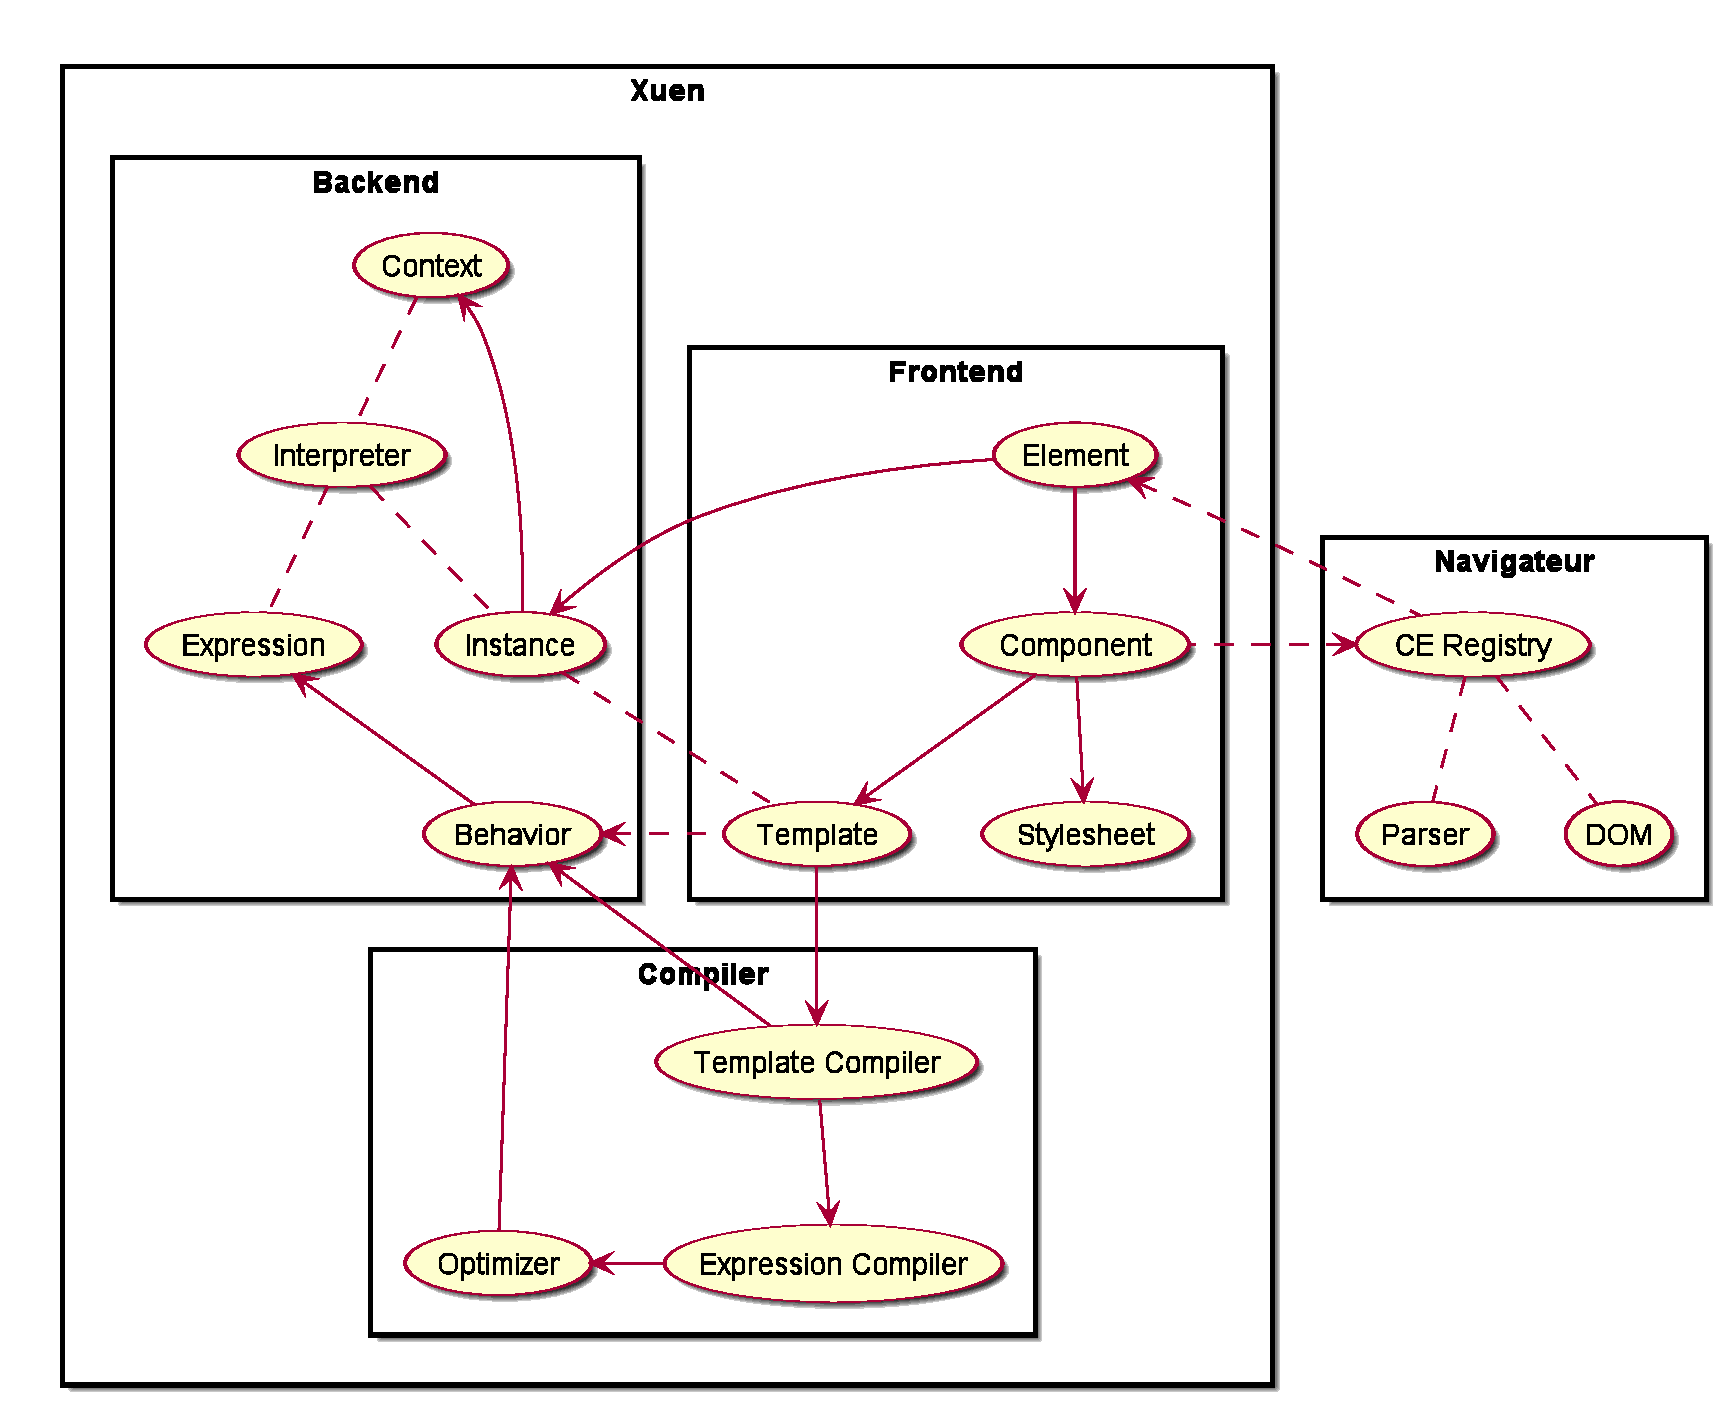
\includegraphics[width=\textwidth]{img/web_overview.eps}
	\caption{Vue d'ensemble de l'implémentation du framework Web}
	\label{fig:web-overview}
\end{figure}

L'implémentation du framework web de Xuen peut être décomposé en 3 grandes parties, tel qu'illustré par la figure \ref{fig:web-overview}.

\begin{enumerate}
	\item La partie \emph{front-end} est exposée directement au développeur. Elle est utilisée pour déclarer les composants personnalisés de l'application, leurs comportement et structure.
	\item La partie \emph{back-end} est utilisée par le framework lorsqu'un élément est instancié dans le document. Elle fournit les outils nécessaires à l'implémentation des comportements dynamiques du template de cet élément et l'interface avec le système de signaux par le biais des expressions.
	\item Finalement le système de compilation est utilisé lors de la définition d'un nouveau composant pour transformer le code source HTML du template en une instance de la classe \texttt{Template}, encapsulant à la fois une structure pré-traitée du template, des modèles pour construire les comportements dynamiques de ce template et des expressions sous forme d'arbres syntaxiques prêts à être interprétés.  
\end{enumerate}

L'objectif de la partie de compilation est de réduire l'impact du traitement du template au \emph{runtime}. En effet, l'instanciation d'un template se base sur les outils fournis par le navigateur, notamment le parser HTML et son implémentation du DOM afin parcourir et traiter la structure fournie sous forme de code HTML.

En compilant le template et les expressions dès la déclaration, il n'est plus nécessaire de le faire lors de l'instanciation, ce qui permet un investissement fixe au chargement de l'application et des performances accrues lors de son fonctionnement.

Cette structure est en grande partie reprise d'un projet personnel antérieur. La plupart des éléments ont été repensés et réimplémentés, principalement pour les adapter au nouveaux standards \emph{Web Components} version \emph{v1} (par opposition à la version antérieure \emph{v0}). Le parser d'expression a quant à lui été réécrit, passant d'une implémentation fortement inspirée du parser d'expression du framework Angular 2, mais en Scala, à une version développée avec la bibliothèque \emph{scala-parser-combinators} \cite{scala-parser-combinators}, plus propre et idiomatique. La grammaire du langage n'a cependant pas été significativement modifiée. L'optimisateur d'expressions est réutilisé pratiquement tel quel.

\subsection{Processus de compilation du template}

Le template est fourni à la bibliothèque sous forme de code source HTML. La première opération consiste donc à construire dynamiquement un élément \texttt{<template>} et à y insérer le code du développeur. Le parser HTML du navigateur sera alors invoqué pour construire une structure de nœuds DOM. Cette structure est ensuite parcourue de façon récursive en commençant à l'élément template créé précédemment.

\begin{itemize}
	\item Premièrement, la nature du noeud en cours est déterminée. S'il s'agit d'un nœud \texttt{Text} ou \texttt{Comment}, son contenu est scanné pour y identifier d'éventuelles interpolations.
	\item Si le nœud est un élément, ses attributs sont observés.
	\item Si l'élément est annoté d'une transformation \texttt{*if} ou \texttt{*for}, cette transformation est appliquée.
	\item Si l'élément possède des annotations de \emph{data-binding}, celles-ci sont traitées.
	\item Les valeurs des attributs restants qui ne sont ni des transformations ni des annotations de \emph{data-binding} sont scannées pour y identifier des interpolations.
	\item Une fois l'élément lui-même entièrement traité, l'ensemble de ses enfants est parcouru, réitérant le processus.
\end{itemize}

Pour chaque nœud DOM devant être associé à un comportement dynamique, un \texttt{Behavior} est créé. Celui-ci est identifié par un numéro incrémenté à chaque nouvelle instance. Il sera de modèle pour la construction du comportement dynamique en question. Tous les \texttt{Behavior}s créés pour un template son rassemblé dans une \texttt{Map} contenue dans l'objet \texttt{Template} resultant. L'élément auquel le comportement doit être attaché est quant à lui décoré d'un attribut \texttt{xuen:behavior="..."} indiquant l'identifiant du comportement associé à ce nœud.

Si l'élément ne peut pas posséder d'attribut, c'est à dire lorsqu'il s'agit d'un nœud \texttt{Text} ou \texttt{Comment}, un élément \emph{placeholder} \texttt{<xuen:placeholder>} est inséré à sa place dans l'arbre DOM du template et l'attribut est placé sur cet élément. Dans ce cas, lors de la construction du comportement au moment de l'instanciation du template, l'élément \emph{placeholder} sera en premier lieu remplacé par un nœud correspondant à l'original puis le comportement spécifique de ce nœud sera implémenté.

Un \texttt{Behavior} peut en réalité implémenter plus d'un comportement pour un même élément. Si deux annotations sont présentes sur un même élément, le \texttt{Behavior} construit à l'occasion du traitement de la première annotation est réutilisé pour la deuxième annotation. L'objet \texttt{Behavior} sera donc en charge de construire deux comportements dynamiques différents sur le même élément.

À l'inverse de la compilation, le processus d'instanciation est relativement simple. Le template est à présent sous forme normalisée, tous les comportements sont attachés à des éléments annotés par l'attribut \texttt{xuen:behavior}. Juste avant d'implémenter les comportements dynamiques, l'objet template est cloné pour construire une nouvelle structure indépendante de l'originale qui est conservée en tant que modèle. La bibliothèque utilise alors la \texttt{Map} associant les identifiants des différents comportements enregistrés avec les objets \texttt{Behavior} encapsulant la logique de construction pour instancier à proprement parler ces comportements.

Le sélecteur CSS \texttt{[xuen:behavior="..."]} est utilisé pour récupérer l'élément sur lequel le comportement doit être appliqué puis la méthode \texttt{build} de l'objet \texttt{Behavior} est invoquée avec la référence vers l'élément courant. Cette méthode va alors instancier à proprement l'ensemble des comportements liés à cet élément.

De façon générale \emph{instancier un comportement} implique construire une paire (signal, observateur) qui implémentera le comportement désiré. Cette paire est initialement construite déconnectée. Une fois l'élément hôte connecté, son template est \emph{activé} ce qui entraine la liaison  des observateurs avec le signal associé et donc la mise en place du comportement dynamique.

Lorsqu'un élément est déconnecté, son template est \emph{désactivé}. Cette opération déconnecte l'ensemble des signaux et observateurs utilisé dans l'implémentation de ce template, assurant ainsi qu'il n'existe plus de lien entre le reste du système et l'élément déconnecté. Sans cette étape, il existe un risque que les éléments ne puissent pas être désalloués par le \emph{garbage collector} puisqu'une référence subsiste entre le reste du graphe de signaux et eux.

\subsection{Ordre de construction des \emph{Custom Elements}}

La spécifique \emph{Custom Elements} \cite{w3c-custom-elements} défini très précisément la façon dont un élément personnalisé est initialisé par le navigateur. Cette procédure, appelée \emph{upgrade} \cite[\small 2.5 Upgrades]{w3c-custom-elements}, implique une combinaison de piles et de queues pour enregistrer les actions à effectuer par le navigateur au fil de l'analyse du document HTML.

De plus la notion de \emph{connexion} au document est introduite: un élément est \emph{connecté} si il fait partie de la hiérarchie du document, \emph{déconnecté} s'il s'agit d'un élément flottant hors de l'arbre DOM principal.

L'\emph{upgrade} d'un élément ne s'effectue en principe que si cet élément est \emph{connecté} au document. Sauf s'il s'agit d'un élément étant explicitement créé par l'utilisateur. Ainsi l'utilisation de la méthode \texttt{createElement} avec un élément personnalisé provoque l'\emph{upgrade} instantané de l'élément créé, mais laisse les éléments de son template dans l'état non-\emph{upgradé}, car ceux-ci n'ont pas été instancié explicitement et que leur parent, en l'occurrence l'élément créé par \texttt{createElement}, n'est pas encore inséré dans le document; ils ne sont donc pas considérés \emph{connectés}.

Le constructeur de l'élément racine est donc invoqué alors que le constructeur de ses enfants n'a pas encore été invoqué. Hors, il est déjà possible d'utiliser \texttt{querySelector} pour accéder à ces éléments non-initialisés.

Le problème s'amplifie lorsque l'élément parent devient \emph{connecté}. Le mécanisme de queues décrit dans le standard implique que l'appel du \emph{callback} de l'élément parent est planifié avant la considération des éléments enfants. Par conséquent, la méthode \texttt{connecteCallback} est invoquée sur l'élément parent, une fois encore, avant que ses enfants n'aient eu l'occasion de s'initialiser.

Dans Xuen, le \emph{callback} de connexion est utilisé pour activer le template de l'élément parent, construisant alors l'ensemble des liens de \emph{data-binding} entre parent et enfants. Si un élément enfant n'est pas encore instancié à ce moment là, les points de connexion sous forme de signaux permettant le \emph{data-binding} ne sont pas encore disponibles et le système est alors laissé dans un état totalement inutilisable.

Afin de contourner ce problème, l'initialisation d'un élément personnalisé place temporairement les éléments de son template dans l'élément \texttt{<body>} du document, forçant ainsi l'\emph{upgrade} de ses éléments enfants. Ces éléments sont par la suite déplacés dans le \emph{Shadow DOM} de l'élément, cette fois-ci dans l'état initialisé. Cette opération s'effectue dans le constructeur de la classe \texttt{Element} du framework, avant le constructeur de la sous-classe implémentée par le développeur. Celui-ci est donc libre d'accéder aux éléments du template du composant avec la garantie que ceux-ci seront initialisés.

Cette sémantique imposée par le standard est déroutante. Le fait de retarder l'\emph{upgrade} d'un élément à sa connexion est déjà étonnant, mais appeler le \emph{callback} de connexion de son parent avant de considérer l'\emph{upgrade} des enfants est réellement problématique.

Le standard conseille de retarder les opérations d'initialisation à la première invocation du \emph{callback} de connexion. Par conséquent, accéder aux éléments enfants lors de l'invocation du constructeur peut sembler être une mauvaise pratique. En revanche, il n'est pas cohérent que ces éléments ne soient toujours pas initialisés au moment où l'élément parent devient connecté. Comment le développeur est-il sensé configurer les composants de son template si ceux-ci ne sont pas encore entièrement construits ?

%\chapter{Haut-niveau}

\section{Signal}

\subsection{Définition}

Un signal de type \texttt{Signal[T]} est l'unité élémentaire d'un système réactif-fonctionnel. C'est un conteneur pour une valeur de type \texttt{T} dont la valeur peut changer au cours du temps, il peut également être \emph{indéfini} et n'est alors associé à aucune valeur au moment présent.

Un signal peut également posséder un nombre quelconque de signaux \emph{parents}, nécessaires à la définition de sa propre valeur. Il peut également être composés à d'autre signaux et transformés par l'application de fonctions afin de produire de nouveaux signaux dérivés.

L'arbre de signaux ainsi construit représente alors un ensemble de transformations fonctionnelles appliquées de façon continue sur les valeurs des signaux sources situés à la racine et permettant d'en dériver les valeurs des signaux feuilles, correspondant aux valeurs utiles à l'application réalisée.

\subsection{Opérations monadiques}

\subsubsection{\texttt{map}}
\subsubsection{\texttt{flatMap}}
\subsubsection{\texttt{filter}}
\subsubsection{\texttt{fold}}

\subsection{Expression}

Signaux expression

\subsection{Comparaison avec les \texttt{Rx} de \emph{ReactiveX}}

Dans les implémentations les plus populaires de framework réactifs-fonctionnels, dont notamment la bibliothèque \emph{ReactiveX} disponible pour de nombreux langages, on retrouve généralement un concept similaire sous le nom de \texttt{Rx}.

Bien que tous deux soient une abstraction du temps, les \texttt{Rx} représentent fondamentalement une séquence tandis qu'un \texttt{Signal} est une valeur unique à un instant donné. Afin de clarifier cette distinction, ces deux interfaces peuvent être comparées à leur équivalent non-réactif le plus proche dans la bibliothèque standard de Scala:

\begin{table}[H]
	\begin{tabular}{@{}p{2.5cm}p{2.5cm}p{\dimexpr\textwidth-6cm\relax}@{}}
		\toprule
		Type de base & Type réactif & Différence \\ \midrule
		\texttt{Stream[T]} & \texttt{Rx[T]} & Tous les éléments d'un \texttt{Stream} sont calculables à l'instant présent, les éléments d'une \texttt{Rx} ne sont peut être pas encore disponibles \\
		&  & \\
		\texttt{Future[T]} & \texttt{Signal[T]} & Un \texttt{Future} n'est résolu qu'une seule fois, un \texttt{Signal[T]} peut changer de valeur de multiples fois au cours du temps \\ \bottomrule
	\end{tabular}
\end{table}

Ainsi, certaines opérations monadique dont la sémantique peut être ambiguë dans le cas des valeurs réactives peuvent avoir des comportements considérablement différents entre ces deux concepts. C'est le cas notamment de la fonction \texttt{flatMap}
\footnote{\texttt{Signal[T].flatMap[U](fn: T => U): Signal[U]}, de façon similaire pour \texttt{Rx[T]}}:

\begin{itemize}
	\item Sur une valeur \texttt{Rx}, l'opération \texttt{flatMap} effectue une concaténation des valeurs des sous-séquences retournées, potentiellement entrelacées.
	\item Sur un \texttt{Signal}, l'opération \texttt{flatMap} se comporte comme un switch: le signal original est utilisé pour sélectionner un second signal, dont la valeur sera celle du signal produit par \texttt{flatMap}. Lorsque la valeur du signal initial change, la sélection est effectuée à nouveau et le signal résultant est utilisé comme nouvelle source de valeurs.
\end{itemize}

Bien que la bibliothèque \emph{ReactiveX} propose un opérateur spécifique avec la sémantique de switch, il est utile de préciser que l'opération \texttt{flatMap} est l'opération utilisée par le langage Scala lors de l'utilisation de multiples générateurs dans une compréhension \texttt{for}.

Ainsi le code
\begin{lstlisting}
val a: Signal[Int] = ...
val b: Array[Signal[Double]] = ...
val c: Signal[Double] = for (x <- a; y <- b(x)) yield y * 2
\end{lstlisting}

sera transformé par le compilateur en
\begin{lstlisting}
val c = a.flatMap(x => b(x)).map(y * 2)
\end{lstlisting}

et produira des résultats radicalement différents selon l'abstraction utilisée:

\begin{itemize}
	\item Dans le cas des \texttt{Rx}, le résultat est l'agglomération des tous les flux de valeurs de \texttt{b} sélectionnés au fil du temps, potentiellement de multiples fois. Le résultat n'est très probablement pas celui escompté.
	
	\item Dans le cas de \texttt{Signal}, le résultat est un signal \texttt{c} dont la valeur est le double de celle d'un signal contenu dans le tableau \texttt{b} et désigné par la valeur du signal \texttt{a}, le tout sur la base des valeurs de ces signaux au moment présent. Dans le future, lorsque la valeur de \texttt{a} ou de \texttt{b(x)} changera, la valeur de \texttt{c} sera également mise à jour.
\end{itemize}

La sémantique des signaux, basée sur les valeurs plutôt que la séquences de ces valeurs, a pour but d'être la plus adaptée possible à l'usage qui en est fait dans ce travail, c'est à dire la conception d'interfaces graphique. Dans cette optique, la sémantique associée à la compréhension \texttt{for} par les signaux semble plus adaptées que la sémantique non-déterministe des \texttt{Rx}.

Une conséquence supplémentaire de cette différence entre signaux et \texttt{Rx} est la possibilité de définir aisément le concept de \emph{signal expression} dans le cas des signaux. Dans le cas des \texttt{Rx}, le comportement attendu d'une telle construction n'est pas évident dans une situation où les flux sont potentiellement finis. \textit{A PRECISER}

\section{Comparaisons}
\section{MonadicHTML}

\section{Framework reactif}

\section{Construction de composants web}
\subsection{Intégration RX et templates}
%\include{tex/priorart}
%\chapter{Xuen: Implémentation}

\section{Signaux}

\subsection{Hiérarchie}
\label{sec:sig-hierarchy}

La figure \ref{sec:sig-hierarchy} présente la hiérarchie formée par les différentes classes de signaux. Cette section aborde plus en détails les spécificités de chacune d'elles.

\begin{figure}[h]
	\centering
	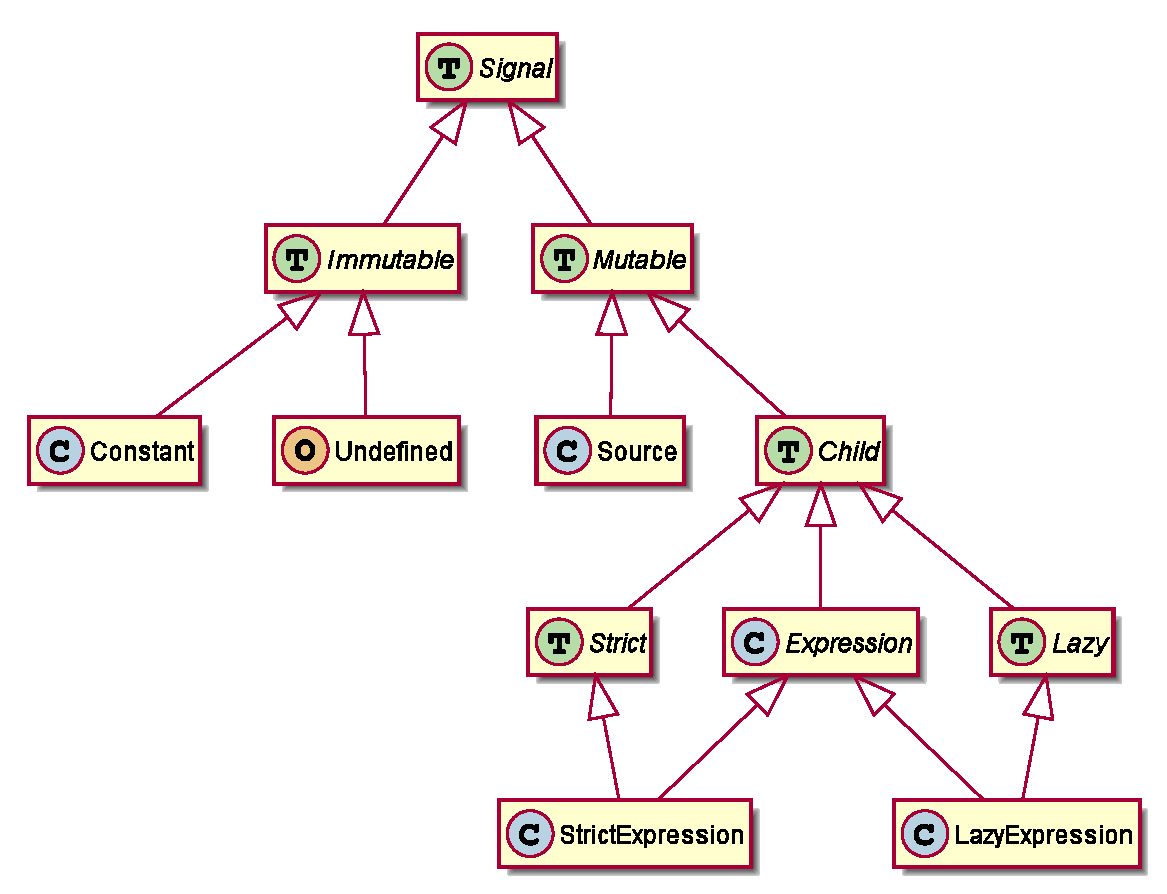
\includegraphics[width=10cm]{img/sig_hierarchy.eps}
	\caption{Hiérarchie des signaux}
	\label{fig:sig-hierarchy}
\end{figure}

\subsubsection{\texttt{Signal}}

Le trait racine de la hiérarchie expose les opérations communes à tous les signaux: accès à la valeur courante et opération de transformation. C'est une interface générique qui ne précise aucune sémantique particulière pour le signal. Elle est ainsi adaptée lorsque le type exact de signal manipulé n'est pas important, ce qui est généralement le cas.

\subsubsection{\texttt{Immutable}}

Cette première division distingue les signaux dont la valeur change au cours du temps de ceux pour lesquels la valeur reste constante.

\subsubsection{\texttt{Mutable}}

\subsubsection{\texttt{Lazy}}

\subsection{Implémentation des opérateurs monadiques}

\textit{CONTRAIREMENT À REACTIVEX, PAS DE CLASSES, MAIS UTILISATION DES EXPRESSIONS}

\subsection{Modèle push, pull ou hybride}

Deux modes de fonctionnement sont généralement décrit pour des systèmes fonctionnels-réactifs: \emph{push} et \emph{pull}.

L'approche \emph{push} se base sur les changements apportés aux signaux sources pour recalculer tous les signaux enfants qui en dépendent. Dans l'approche \emph{pull}, c'est l'accès aux signaux enfants qui provoque le calcul des valeurs intermédiaires jusqu'aux signaux sources. Dans les deux cas, des opérations potentiellement inutiles ou redondantes sont effectuées.

L'approche mixte \emph{push-pull} se base sur une approche principalement \emph{pull} où l'accès à l'état d'un signal déclenche son évaluation, auquel vient s'ajouter un mécanisme de \emph{mémoïsation} qui maintient l'état courant du signal après son calcul. L'invalidation de ces caches se fait ensuite selon une approche \emph{push}: un changement d'état des signaux sources est notifié à toutes les dépendances de façon récursive.

\textit{DEVELOPPEMENT DES AVANTAGES}

\subsection{Utilisation dans un environnement parallèle}

\textit{Pas de threads en JavaScript, donc un problème que côté serveur. Bien que le système fonctionne sur la JVM, il n'a pas été testé de façon étendue dans un contexte multi-thread; actuellement half-baked: les Signaux eux-même sont en principe thread-safe (aka invalidation / recalcul / etc) mais le système en entier n'est pas réellement étudié (dead-lock de signaux interdépendant?). Est-ce que utile au projet puisqu'on le use-case principal est celui du framework web côté client? Quid des observeurs et de la sémantique exactly-once pour une bloc de mutation atomic{} ?}

\section{Framework web}


\part{Application Guild-Tools}
\chapter{GuildTools}

\textit{Note: Cette section décrit très brièvement l'application GuildTools qui sera développée en utilisant le framework réactif-fonctionnel. La liste de fonctionnalités correspond aux fonctionnalités prévues au moment de ce rapport intermédiaire. Ces fonctionnalités peuvent être amenées à varier d'ici au rendu final. }

\section{Objectif}

Application de gestion de guilde sur World of Warcraft.

\section{Fonctionnalités}

	\subsection{Profil de joueur}

	Ce premier module est destiné à collecter et gérer l'ensemble des données de profil d'un joueur: son nom et prénom, son age, ses informations de contact en jeu ainsi que ses différents personnages.

	\subsection{Calendrier}
	
	Un calendrier partagé permettant de définir les soirées de jeu de l'équipe. 
	
	Chaque événement offre une liste des joueurs enregistrés comme présents ou absents, ainsi qu'une note optionnelle permettant au joueur d'apporter des précisions supplémentaires.
	
	Un système de gestion des absences de façon globale est aussi disponible, permettant aux joueurs de définir des plages pendant lesquels ils sont indisponibles à tous les événements créés ou futurs.
	
	\subsection{Roster}
	
	Une vue d'ensemble des joueurs du groupe et de leurs personnages avec la possibilité de filtrer selon différents critères.
	
	\subsection{Whishlists}
	
	Un module permettant de saisir les besoins des différents personnages d'un joueur, facilitant ainsi la composition des groupes par les officiers.
	
	\subsection{Composition de groupes}
	
	Un module simplifiant la construction de groupe de jeu en s'assurant qu'un joueur ne se trouve pas simultanément dans plusieurs groupes. Ces groupes sont ensuite exportables vers un événement calendrier.
	

\part{Annexes}
\appendix

%\chapter{Cahier des charges}

Ce travail de Bachelor a pour objectif de concevoir une application de gestion collaborative qui permet à ses utilisateurs d'interagir en temps réel pour accomplir certaines tâches (organisation du groupe, gestion des membres, gestion des scores, etc.)

\begin{enumerate}
	\item Conception d'un modèle de données
	
	\item  Conception d'une architecture et d'un protocole pour la propagation des données en temps réel entre serveur et clients
	
	\item  Conception d'une couche de présentation qui reflète en temps réel le modèle de données dans un document HTML
	
	\item  Développement d'une application web (client et serveur) avec programmation en paradigme réactif et fonctionnel (Scala, Scala.js)
\end{enumerate}

Dans la conception l'accent sera mis sur le développement de structures réutilisables dans d'autres applications collaboratives.

%\chapter{Journal de travail}

\textit{Note: ce journal de travail n'ayant pas été demandé initialement, il a été réalisé à postériori sur la base de l'historique des dépôts Git de ce document et de la bibliothèque réactive-fonctionnelle.} Oops, I forgot! I bet that Graf forgot it too!
\chapter{Grammaire des expressions}

Cette section décrit la grammaire des expressions utilisées dans les templates Xuen. La syntaxe utilisée correspond à la syntaxe définie par le W3C pour la description de XML \cite{xml-ebnf}. Les notations \texttt{?}, \texttt{+} et \texttt{*}, indiquent respectivement \emph{0-1}, \emph{1-*} ou \emph{0-*} répétitions, de façon similaire à leur signification dans les expressions régulières.

La grammaire ci-dessous inclue simultanément les éléments décomposés entre le \emph{lexer} et le \emph{parser} au niveau de l'implémentation. Les productions notées \texttt{/.../} correspondent à une expression régulière et sont en principe une règles implémentée au niveau du \emph{lexer}.

\subsubsection{Grammaire}
\begin{lstlisting}
expression ::= <empty> | chain

enumerator ::=
	( identifier "," )? identifier "of" simpleExpr
	( "by" simpleExpr )? ( "if" simpleExpr )? ( "with" chain )?

identifier ::= /[a-zA-Z_$][a-zA-Z0-9_$]*/

chain ::= ";"* pipe ( ";"+ ( <empty> | pipe ) )*

pipe ::= simpleExpr ( "|" identifier ( ":" simpleExpr )* )*

simpleExpr ::= conditional

conditional ::= logicalOr ( "?" conditional ":" conditional )?

logicalOr ::= logicalAnd ( "&&" logicalAnd )*

logicalAnd ::= equality ( "||" equality )*

equality ::=
	relational ( ( "==" | "!=" | "===" | "!==" ) relational )*

relational ::= range ( ( "<" | ">" | "<=" | ">=" ) range )*

range ::= additive ( "to" additive ( "by" additive )? )?

additive ::= multiplicative ( ( "+" | "-" ) multiplicative )*

multiplicative ::= prefix ( ( "*" | "/" | "%" ) prefix )*

prefix ::= ( "+" | "-" | "!" )* secondary

secondary ::= primary secondaryAccess*

secondaryAccess ::= memberAccess | bracketAccess | functionCall
memberAccess ::= unsafeMember | safeMember
unsafeMember ::= "." ( memberWrite | memberRead )
safeMember ::= "?." memberRead
memberWrite ::= identifier "=" simpleExpr
memberRead ::= identifier

bracketAccess ::= "[" simpleExpr "]" ( "=" simpleExpr )?

functionCall ::= "(" callArguments ")"

callArguments ::= ( simpleExpression ( "," simpleExpression )* )?

primary ::= parentheses | selector | literal | reference

parentheses ::= "(" chain ")"

selector ::= simpleSelector | complexSelector
simpleSelector ::= /#[a-zA-Z0-9_\-]+/
complexSelector ::= /@\([^)]+\)/

literal ::= keywordLiteral | numberLiteral | stringLiteral | arrayLiteral | objectLiteral

keywordLiteral ::= "undefined" | "null" | "false" | "true"

numberLiteral ::= hexInteger | octInteger | binInteger | decNumber
hexInteger ::= /0[xX][0-9a-fA-F]+/
octInteger ::= /0[oO][0-7]+/
binInteger ::= /0[bB][01]+/
decNumber ::= /((0|[1-9][0-9]*)(\.[0-9]+)?|\.[0-9]+)([eE][+\-]?[0-9]+)?/

stringLiteral ::=
	/:"[^"\\]*(?:\\[\s\S][^"\\]*)*"/ | /'[^'\\]*(?:\\[\s\S][^'\\]*)*'/

arrayLiteral ::=
	"[" (simpleExpression ( "," simpleExpression )* )? "]"

objectLiteral ::= "{" ( objectEntry ( "," objectEntry )* )? "}"
objectEntry ::= objectKey ":" simpleExpr
objectKey ::= identifier | stringLiteral | dynamicKey
dynamicKey ::= "[" simpleExpr "]"
\end{lstlisting}

\chapter{Définition théorique des signaux}
	
\textit{Cette section, rédigée à l'occasion du premier draft de spécification des signaux, constitue une tentative de définition formelle des signaux. Elle est pour l'instant conservée sous forme d'annexe tandis que la spécification des signaux est maintenant construite à partir de son implémentation concrète.}
\vspace{0.5cm}
	
Les signaux sont des constructions fonctionnelles semi-pures. Puisqu'ils encodent la notion de variabilité, ils sont naturellement dépendant du temps en tant qu'état global. Plus spécifiquement, ils dépendent d'un \emph{indice de génération} spécifique à ce signal désigné par $\gamma_s \in \Gamma_s$ qui est associé à chaque changement potentiel d'état du signal.

Dans le cas d'un signal enfant, l'indice de génération est défini comme un $n$-uplet constitué des indices de générations de chaque signaux parents sur lesquels il est dépendant. De cette façon, l'indice et donc l'état des signaux parent est encodé dans l'indice du signal enfant et la dépendance vers d'autres signaux ne compromet pas sa pureté:
\[
	\mathbb{D}^\gamma_{child} = \{ a, b, \dots \} \implies \Gamma_{child} = \Gamma_a \times \Gamma_b \times \dots
\]
avec $\mathbb{D}^\gamma_{a}$ l'ensemble des signaux envers lesquels $a$ est dépendant pour l'indice de génération \gamma. Par définition $|\mathbb{D}^\gamma_{a}| > 0 \iff a$ est un signal enfant.

Dans le cas d'un signal source, l'indice de génération est une valeur abstraite et distincte pour chaque changement d'état.
\[
	\mathbb{D}^\gamma_{source} = \emptyset \implies \forall \alpha \in \Gamma_{source}, \forall \beta \in Signals, (\alpha \notin \Gamma_\beta) \lor (\beta = source)
\]
Un signal peut alors être considéré comme une fonction pure $\Gamma_{sig} \to State_{[T]}$ associant à un indice de génération spécifique un état précis dont la valeur, si elle est définie, est de type $T$.
\[
	sig(\gamma_{sig})\colon \Gamma_{sig} \to State_{[T]} = state \in \{ Undefined, Defined_{[T]}(value) \}
\]
Les changements d'état d'un signal sont des événements séquentiels. L'ensemble des indices de génération de ce signal forment ainsi un ensemble ordonné sur lequel il est possible de définir la fonction
\begin{align*}
	\gamma^*_{sig} = prev(\gamma_{sig}) &\colon \Gamma_{sig} \to \Gamma_{sig}\\
	& = \begin{cases}
		\gamma^*_{sig} & \text{si }
		 \exists \gamma^*_{sig}, \forall \gamma^\alpha_{sig} < \gamma_{sig}, (\gamma^\alpha_{sig} \leq \gamma^*_{sig})\\
		\varnothing & \text{sinon}
	\end{cases}
\end{align*}
associant à chaque indice $\gamma_{sig}$ l'indice $\gamma^*_{sig}$ associé à l'état qui précédait immédiatement l'état associé à l'indice $\gamma_{sig}$. Cette propriété autorise un signal à être défini non seulement en fonction des états actuels d'autres signaux, mais aussi de leurs états antérieurs.

\begin{figure}
	\begin{align*}
		hold (sig) &\colon Signal_{[T]} \to Signal_{[T]} \\
          &\colon (\Gamma_{sig} \to State_{[T]}) \to \Gamma_{sig} \to State_{[T]} \\
          &= \gamma \mapsto \begin{cases}
		           		sig(\gamma) & \text{si } sig(\gamma) \text{ est défini} \\
		           		hold(sig)(\gamma^*) & \text{sinon si } \gamma^* \ne \varnothing \\
		           		Undefined & \text{sinon}
          \end{cases}
	\end{align*}
	\caption{Définition de la fonction $hold$}
	\label{fig:sig-hold}
\end{figure}

\begin{figure}
	\begin{lstlisting}
def hold[T](parent: Signal[T]): Signal[T] = {
	var previous: Option[T] = None
	Signal {
		val state = parent.option
		if (state.isDefined) previous = state
		state orElse previous
	}
}
	\end{lstlisting}
	\caption{Implémentation de la fonction $hold$}
	\label{fig:sig-hold-scala}
\end{figure}

La figure \ref{fig:sig-hold} présente la définition d'une fonction $hold$ exploitant ce mécanisme pour construire un signal enfant qui maintient sa valeur lorsque son parent devient indéfini.

En pratique, le concept d'indice de génération est implicite. L'accès à un signal se fait toujours à partir de son état le plus récent et la disponibilité des états antérieurs est implémenté en utilisant des variables encapsulées dans le contexte de définition du signal. Les constructions ainsi formées ne sont donc pas strictement pures d'un point de vue fonctionnel mais sont compatible avec la notion théorique d'un signal et ne causent pas de surprise lors à l'usage. La figure \ref{fig:sig-hold-scala} présente une implémentation possible de la fonction $hold$ en Scala.

En résumé, les fonctions utilisées pour définir ou transformer un signal doivent être \emph{semi-pures}:
\begin{enumerate}
	\item elles ne peuvent dépendre d'aucun état implicite, hormis d'autres signaux et leurs états antérieurs, et
	\item elles ne doivent pas contenir d'effets de bords observables
\end{enumerate}
De cette façon, l'ordre d'évaluation des signaux ou même leur évaluation différée n'a pas d'importance dans le comportement du système. Ces propriétés ne sont pas vérifiables au niveau du langage, le développeur est ainsi responsable de s'assurer que ses fonctions soient conformes à ces contraintes.

Le concept d'\emph{observateur} (Section \ref{sec:sig-obs}) est un mécanisme permettant d'introduire des effets de bords à partir de signaux, de façon sûre et définie.

\section*{Opérations élémentaires}

	\subsection*{Sélection (flatMap)}
		
		\begin{align*}
			flatMap(a, f)
				&\colon (Signal_{[T]}, T \to Signal_{[U]}) \to Signal_{[U]} \\
				&\colon (\Gamma_a \to State_{[T]}, T \to \Gamma_f \to State_{[U]}) \to \Gamma_{a \times f} \to State_{[U]} \\
				&= \gamma \mapsto \begin{cases}
					f(v)(\gamma_f) & \text{si } a(\gamma_a) = Defined(v)\\
					Undefined & \text{sinon}\\
				\end{cases}
		\end{align*}
	
	\subsection*{Application (map)}
		
		\begin{align*}
			map(a, f)
				&\colon (Signal_{[T]}, T \to U) \to Signal_{[U]} \\
				&\colon (\Gamma_a \to State_{[T]}, T \to U) \to \Gamma_a \to State_{[U]} \\
				&= flatMap \big( a, v \mapsto \gamma \mapsto Defined(f(v)) \big)\\
				&= \gamma \mapsto \begin{cases}
					Defined \big(f (v) \big) & \text{si } a(\gamma) = Defined(v)\\
					Undefined & \text{sinon}\\
				\end{cases}
		\end{align*}
	
	\subsection*{Filtrage (filter)}
	
		\begin{align*}
			filter(a, p)
				&\colon (Signal_{[T]}, T \to Boolean) \to Signal_{[T]} \\
				&\colon (\Gamma_a \to State_{[T]}, T \to Boolean) \to \Gamma_a \to State_{[T]} \\
				&= flatMap \left( a, v \mapsto \gamma \mapsto \begin{cases}
					a(\gamma) & \text{si } p(v)\\
					Undefined & \text{sinon}\\
				\end{cases} \right)\\
				&= \gamma \mapsto \begin{cases}
					a(\gamma) & \text{si } a(\gamma) = Defined(v) \text{ et } p(v)\\
					Undefined & \text{sinon}\\
				\end{cases}
		\end{align*}
		
	\subsection*{Lecture}
	
		\[
			a.option = \begin{cases}
				Some(a.value) & \text{si } a \text{ est défini}\\
				None & \text{si } a \text{ est indéfini}
			\end{cases}
		\]
		\[
			a.value = \left(opt \mapsto \begin{cases}
				value & \text{si } opt \text{ est } Some(value)\\
				Nothing & \text{si } opt \text{ est } None
			\end{cases}\right) \circ a.option
		\]




\begin{thebibliography}{99}

\bibitem{odersky2012}
Ingo Maier et Martin Odersky, 2012.
\emph{Deprecating the Observer Pattern with Scala.React}.
EPFL-REPORT-176887\\
\url{https://infoscience.epfl.ch/record/176887}

\bibitem{scala-react}
Ingo Maier, 2012.
\emph{Scala.react is a reactive programming library for Scala}.\\
\url{https://github.com/ingoem/scala-react}

\bibitem{scala.rx}
Li Haoyi et al., 2012--2016.
\emph{scala.rx: An experimental library for Functional Reactive Programming in Scala}.
[Consulté le 24 février 2017]\\
\url{https://github.com/lihaoyi/scala.rx}

\bibitem{haskell-monad-laws}
HaskellWiki.
\emph{Monad laws}.
[Consulté le 24 février 2017]\\
\url{https://wiki.haskell.org/Monad_laws}

\bibitem{czaplicki}
Evan Czaplicki, 2012.
\emph{Elm: Concurrent FRP for Functional GUIs}.
\\
\url{https://www.seas.harvard.edu/sites/default/files/files/archived/Czaplicki.pdf}

\bibitem{czaplicki}
Conal Elliott, 2009.
\emph{Push-Pull Functional Reactive Programming}.
Haskell Symposium\\
\url{http://conal.net/papers/push-pull-frp}

\end{thebibliography}

\end{document}